\documentclass[11pt,review,3p]{elsarticle}

%%\documentclass[final,1p,times]{elsarticle}
%%\documentclass[final,1p,times,twocolumn]{elsarticle}
%%\documentclass[final,3p,times]{elsarticle}
%%\documentclass[final,3p,times,twocolumn]{elsarticle}
%%\documentclass[final,5p,times]{elsarticle}
%%\documentclass[final,5p,times,twocolumn]{elsarticle}

\usepackage{amssymb}
\usepackage{amsmath}
\usepackage{lineno}
\usepackage[utf8]{inputenc}
\usepackage[per-mode=symbol]{siunitx}
\usepackage[colorlinks,bookmarksopen,bookmarksnumbered,citecolor=red,urlcolor=red]{hyperref}
\usepackage{textcomp}
\usepackage{multirow}
\usepackage{xcolor, soul}
\usepackage{caption}
\usepackage{subcaption}
\usepackage{siunitx}
\usepackage{booktabs}
\sethlcolor{green}
\usepackage{physics}
\usepackage{cleveref}
\usepackage{graphicx}
\graphicspath{{figures/}}
\usepackage{enumitem}
\usepackage{longtable}
\usepackage{float}
\usepackage{multicol}
\usepackage{fancybox}
\usepackage{afterpage}
\usepackage{nomencl}
\makenomenclature

\renewcommand{\nompreamble}{\vspace{-3em}} % Reduces space after title to "hide" it
% Reduce vertical spacing between items in the nomenclature
\setlength{\nomitemsep}{-0.7em} % Adjust this value to control spacing
%% This code creates the groups
% -----------------------------------------
\usepackage{etoolbox}
\renewcommand\nomgroup[1]{%
  \item[\bfseries
  \ifstrequal{#1}{A}{}{%
  \ifstrequal{#1}{B}{Greek symbols}{%
  \ifstrequal{#1}{C}{Subscripts}{%
  \ifstrequal{#1}{D}{Abbreviations}{}}}}%
]}

% Define a new floating environment for the nomenclature
\newcommand{\nomenclaturebox}{%
  \begin{table*}[!t] % Use table* for spanning both columns
    \centering
    \setlength{\fboxsep}{5pt} % Adjust padding inside the box
    \doublebox{% Creates a double border
      \begin{minipage}{\textwidth}
        \begin{multicols}{2} % Two columns inside the box
          \printnomenclature
        \end{multicols}
      \end{minipage}
    }
  \end{table*}
}

\AtBeginDocument{\RenewCommandCopy\qty\SI}
\ExplSyntaxOn
\msg_redirect_name:nnn { siunitx } { physics-pkg } { none }
\ExplSyntaxOff

\DeclareSIUnit\MWh{MWh}
\DeclareSIUnit\MJ{MJ}
\DeclareSIUnit\cp{\frac{kJ}{kg\cdot K}}
\DeclareSIUnit\eden{\frac{kWh}{m^{3}}}
\DeclareSIUnit\GWht{GWh_{th}}
\DeclareSIUnit\kWht{kWh_{th}}
\DeclareSIUnit\cubicM{m^{3}}
\DeclareSIUnit\kgs{\frac{kg}{s}}
\DeclareSIUnit\globalU{\frac{W}{m^{2}K}}

\journal{Journal of Energy Conversion and Management}

\begin{document}

\begin{frontmatter}

\title{Process Heat Delivery Through Concentrating Solar and Stratified Packed Bed Thermal Energy Storage: A Case Study For The Galvanization Process}

\author[PUC]{Ian Wolde}
\author[UTFSM]{Eduardo González-Mora}
\author[UTEM]{Felipe G. Battisti}
\author[PUC]{Rodrigo Escobar}
\author[PUC,SERC,CDA]{José M. Cardemil}

\affiliation[PUC]{organization={Department of Mechanical and Metallurgical Engineering, Pontificia Universidad Catolica de Chile}, city={Santiago}, country={Chile}}
\affiliation[UTFSM]{organization={Department of Mechanical Engineering, Universidad Técnica Federico Santa María}, city={Valparaíso}, country={Chile}}
\affiliation[UTEM]{organization={Department of Mechanical Engineering, Universidad Tecnológica Metropolitana}, city={Santiago}, country={Chile}}
\affiliation[SERC]{organization={Solar Energy Research Center, SERC Chile}, city={Santiago}, country={Chile}}
\affiliation[CDA]{organization={Centro del Desierto de Atacama, Pontificia Universidad Católica de Chile}, city={Santiago}, country={Chile}}


\begin{abstract}
This work presents a dynamic simulation framework for a concentrating solar thermal plant designed to supply industrial process heat to a hot-dip zinc galvanizing facility. Two plant topologies are compared: Parallel/Indirect (PI), in which the storage is thermally decoupled via heat exchangers, and Series/Direct (SD), in which Solar Salt flows in a single loop through two packed-bed thermal energy storage (PBTES) vessels in series with the process. The packed bed is modeled with the one-dimensional two-phase Schumann equations solved analytically using an eigenvalue decomposition, coupled quasi-steadily to a TESPy thermodynamic network at each hourly timestep. A dynamic lumped-capacitance model of the 150\,000 kg zinc bath provides realistic transient process heat demand. A 144-job full-year parametric sweep covering solar multiples from 0.5 to 3.5, tank geometries spanning 57 to 3{,}770\,m$^3$, physical sensitivities, and a Solar Salt versus Air comparison was completed with 94.4\% success and 100\% timestep convergence. At the baseline design (1\,000\,m$^2$ aperture, $D=7$\,m, $H=5$\,m), the SD topology achieves a solar fraction of 41.3\% against 36.2\% for PI. At a solar multiple of 3.0, SD reaches 80.2\% solar fraction with a levelized cost of heat of approximately \$12/MWh. Physical sensitivity analysis confirms that variations of $\pm20\%$ in particle diameter, void fraction, or insulation thickness alter the annual solar fraction by less than 1 percentage point, demonstrating that the design is robust to packed-bed parameter uncertainty.
\end{abstract}

\begin{keyword}
\sep Thermal Energy Storage \sep Packed Bed \sep Process Heat \sep Concentrating Solar Thermal \sep Galvanizing \sep Solar Salt \sep Levelized Cost of Heat
\end{keyword}

\end{frontmatter}

\linenumbers


\nomenclaturebox

%% main text
\section{Introduction}
\label{sec:Intro}
Galvanized steel is a crucial material for construction across several industries. The galvanization process consists in applying a coat of zinc to steel pieces, to increase durability and avoid corrosion. The coating is typically applied through a hot dip process, which consists of a pool of molten zinc, that must be maintained at a temperature of \SI{450}{\celsius} by using gas burners to control the temperature \cite{Blakey2004-sl}.

The galvanizing industry can be included in the decarbonization pathways, as the use of fossil fuel could be replaced by clean energies. Due to the high temperature of the process, concentrating solar thermal systems are ideal, as they can deliver heat at the required temperature. Dedicated heat transfer fluids (HTF) must be assessed, that can work at high temperatures. Molten salts \cite{Bonini2024-za} and supercritical CO2 \cite{Battisti2022-nw} have been evaluated with successful results.

Thermal energy storage (TES) systems can increase the technical and economic viability of the solar thermal system, especially when using packed-bed (PBTES) technology \cite{Battisti2021-wv}. Furthermore, solid-state TES such as packed-bed technology presents a high compatibility with metallurgical industry, due to the high temperature in the processes' heat demand (Wolde, \cite{Wolde2024-dm}).

\section{Methodology}
\label{sec:Methodology}

\subsection{System Description}
\label{sec:sys_desc}

The present study evaluates a solar thermal plant designed to supply industrial process heat to a hot-dip galvanizing facility. The plant comprises three main subsystems, as illustrated in Fig.~\ref{fig:plant_layout}: a parabolic trough collector (PTC) solar field, a packed bed thermal energy storage (PBTES) unit, and a dynamic zinc galvanizing bath. Two principal configurations are compared:

\begin{figure*}[!htbp]
    \centering
    \begin{subfigure}[b]{0.49\textwidth}
        \centering
        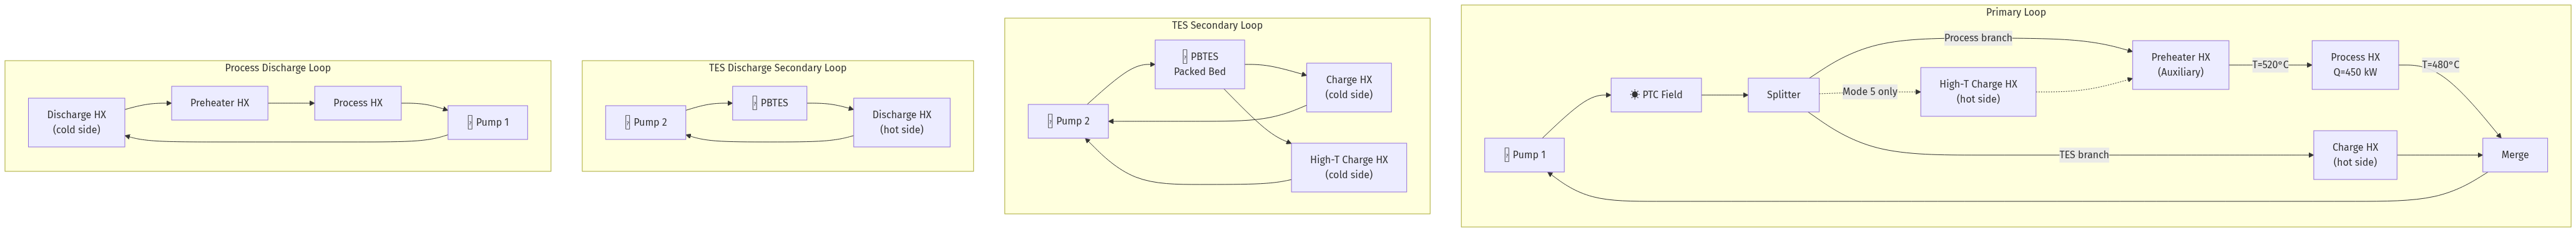
\includegraphics[width=\linewidth]{fig01a_layout_pi.png}
        \caption{Parallel / Indirect (PI) Configuration}
        \label{fig:layout_pi}
    \end{subfigure}
    \hfill
    \begin{subfigure}[b]{0.49\textwidth}
        \centering
        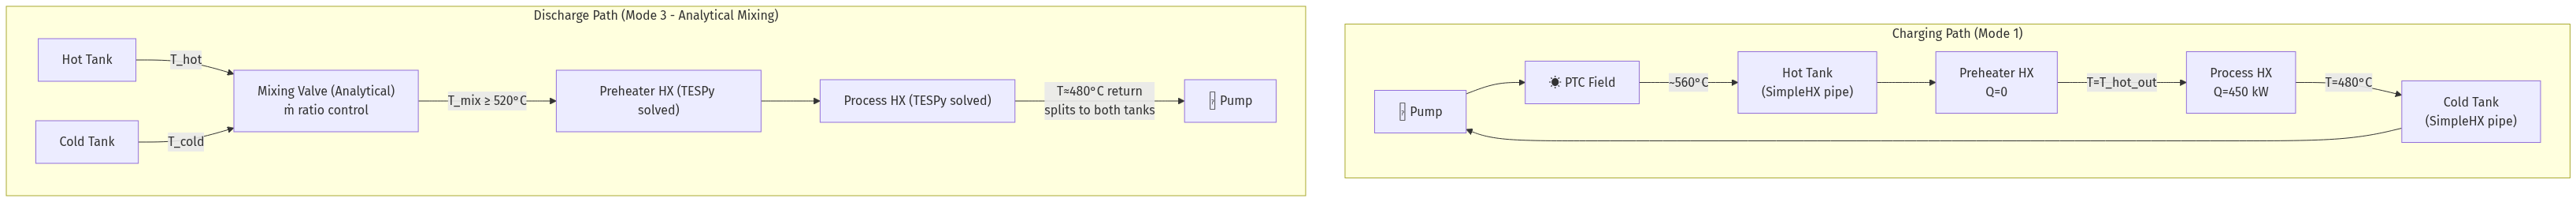
\includegraphics[width=\linewidth]{fig01b_layout_sd.png}
        \caption{Series / Direct (SD) Configuration}
        \label{fig:layout_sd}
    \end{subfigure}
    \caption{Schematic diagrams of the two plant topologies compared in this study: (a) Parallel/Indirect (PI) baseline layout showing primary, secondary charging, secondary discharge, and process loops; (b) Series/Direct (SD) configuration showing charging path (Mode 1) and parallel discharge path with analytical mixing valve (Mode 3).}
    \label{fig:plant_layout}
\end{figure*}

\begin{enumerate}[label=\textbf{(\Alph*)}, leftmargin=*]
    \item \textbf{Parallel / Indirect (PI)} --- The baseline layout. The heat transfer fluid (HTF) leaving the PTC field can split between a process heat exchanger and a dedicated charging heat exchanger (HX) that couples the primary loop to a secondary TES loop. A separate discharge HX connects the storage loop to the process preheater. This configuration decouples HTF inventories, operating pressures, and flow paths.
    \item \textbf{Series / Direct (SD)} --- A sequential single-loop configuration. The primary Solar Salt flows directly through two packed-bed storage vessels placed in series: a Hot Tank upstream of the process (receiving full PTC outlet temperature at approximately \SI{560}{\celsius}) and a Cold Tank downstream of the process (receiving the process return at approximately \SI{480}{\celsius}). No intermediate heat exchangers are used between the primary loop and the storage.
\end{enumerate}

The primary HTF is Solar Salt (a commercial sodium--potassium nitrate mixture), modeled via the CoolProp library as \texttt{INCOMP::NaK}. The fluid operates within a temperature envelope of \SIrange{300}{600}{\celsius}, constrained by freezing at the lower bound and thermal degradation at the upper bound. For parametric comparison, a low-cost reference fluid (Air) is also evaluated.

The plant is driven by hourly weather data from a Typical Meteorological Year (TMY) file for Santiago, Chile, providing direct normal irradiance ($E$, \si{W.m^{-2}}) and dry-bulb ambient temperature ($T_{\text{amb}}$, \si{\celsius}) at each timestep.

\subsection{Mathematical and Physical Models}
\label{sec:physics}

\subsubsection{Parabolic Trough Collector Solar Field}
\label{sec:ptc_model}

The PTC solar field converts direct normal irradiance into useful thermal power delivered to the HTF. The net thermal power output $\dot{Q}_{\text{ptc}}$ is:

\begin{equation}
    \dot{Q}_{\text{ptc}} = A_{\text{ptc}} \left[ E \cdot \eta_{\text{opt}} \cdot K(\theta) - \dot{q}_{\text{losses}} \right]
    \label{eq:ptc_power}
\end{equation}

where $A_{\text{ptc}}$ is the total collector aperture area (\SI{1000}{m^2} at the baseline design point, with parametric sweeps covering \SIrange{500}{3000}{m^2}), $E$ is the DNI from the weather file, and $\eta_{\text{opt}} = 0.816$ is the design-point optical efficiency accounting for mirror reflectivity, glass envelope transmissivity, and absorber tube absorptivity.

The incident angle modifier $K(\theta)$ corrects for optical losses at non-normal solar incidence angles $\theta$ (in degrees):

\begin{equation}
    K(\theta) = 1 + i_{1}\, \theta + i_{2}\, \theta^{2}
    \label{eq:iam}
\end{equation}

with coefficients $i_{1} = \num{-1.59e-3}\ \si{deg^{-1}}$ and $i_{2} = \num{9.77e-5}\ \si{deg^{-2}}$.

Area-specific thermal losses $\dot{q}_{\text{losses}}$ from the receiver tube to the environment are modeled as:

\begin{equation}
    \dot{q}_{\text{losses}} = c_{1} \left(T_{\text{ptc,avg}} - T_{\text{amb}}\right) + c_{2} \left(T_{\text{ptc,avg}} - T_{\text{amb}}\right)^{2}
    \label{eq:ptc_loss}
\end{equation}

with $c_{1} = \SI{0.0622}{W.m^{-2}.K^{-1}}$ and $c_{2} = \SI{0.00023}{W.m^{-2}.K^{-2}}$, and $T_{\text{ptc,avg}} = (T_{\text{ptc,in}} + T_{\text{ptc,out}})/2$.

The PTC field is modeled within the TESPy thermodynamic network as a standard parabolic trough component, which solves for the outlet temperature and mass flow rate as part of the full system energy balance at each timestep.

\subsubsection{Heat Transfer Fluid}
\label{sec:htf}

The primary HTF, Solar Salt, is represented in CoolProp as \texttt{INCOMP::NaK}. Its temperature-dependent thermophysical properties --- density (from approximately \SI{1900}{kg.m^{-3}} at \SI{300}{\celsius} to \SI{1700}{kg.m^{-3}} at \SI{600}{\celsius}), specific heat capacity (on the order of \SI{1500}{J.kg^{-1}.K^{-1}}), thermal conductivity (approximately \SI{0.53}{W.m^{-1}.K^{-1}}), and dynamic viscosity --- are evaluated at each timestep via the CoolProp property database. The simulation clamps the fluid temperature to a working range between \SI{300.1}{\celsius} (preventing freezing and numerical property evaluation failures) and \SI{600}{\celsius} (preventing thermal degradation).

\subsubsection{Packed Bed Thermal Energy Storage}
\label{sec:pbtes_model}

The TES tank consists of a cylindrical packed bed of solid rock or ceramic pebbles with the geometric and material properties listed in Table~\ref{tab:tes_params}. The heat transfer between the fluid and solid phases is modeled using the classical one-dimensional Schumann equations:

\begin{align}
    \frac{\partial T_f}{\partial t} + u \frac{\partial T_f}{\partial z} &= \frac{h_v}{\rho_f c_{p,f} \varepsilon} \left(T_s - T_f\right) - \frac{U_{\text{tank}} P}{\rho_f c_{p,f} A_{\text{bed}} \varepsilon} \left(T_f - T_{\text{amb}}\right) \label{eq:schumann_f} \\
    \frac{\partial T_s}{\partial t} &= \frac{h_v}{\rho_s c_{p,s} (1 - \varepsilon)} \left(T_f - T_s\right) \label{eq:schumann_s}
\end{align}

where $z$ is the axial coordinate along the bed height ($0 \le z \le H$), $u = \dot{m} / (\rho_f A_{\text{bed}} \varepsilon)$ is the interstitial fluid velocity, and $U_{\text{tank}} = \SI{0.15}{W.m^{-2}.K^{-1}}$ is the tank overall heat loss coefficient to ambient.

The volumetric heat transfer coefficient $h_v$ is derived from the particle-scale convection coefficient $h_{sf}$:

\begin{equation}
    h_v = \frac{6 (1 - \varepsilon)}{d_p} h_{sf}
    \label{eq:hv}
\end{equation}

where $h_{sf}$ is obtained from the Wakao--Kaguei correlation for packed beds:

\begin{equation}
    Nu = \frac{h_{sf} d_p}{k_f} = 2.0 + 1.1\, Re^{0.6} Pr^{1/3}
    \label{eq:wakao}
\end{equation}

\begin{table}[h]
\centering
\caption{Packed bed TES geometric and material parameters.}
\label{tab:tes_params}
\begin{tabular}{lll}
\toprule
Parameter & Symbol & Value \\
\midrule
Tank height & $H$ & \SI{5.0}{m} \\
Tank diameter & $D$ & \SI{7.0}{m} \\
Particle diameter & $d_p$ & \SI{0.050}{m} \\
Void fraction & $\varepsilon$ & 0.40 \\
Solid density & $\rho_s$ & \SI{3500}{kg.m^{-3}} \\
Solid specific heat & $c_{p,s}$ & \SI{968}{J.kg^{-1}.K^{-1}} \\
Solid thermal conductivity & $k_s$ & \SI{1.6}{W.m^{-1}.K^{-1}} \\
Insulation thickness & $\delta_{\text{ins}}$ & \SI{1.0}{m} \\
Insulation conductivity & $k_{\text{ins}}$ & \SI{0.012}{W.m^{-1}.K^{-1}} \\
Tank overall heat loss coeff. & $U_{\text{tank}}$ & \SI{0.15}{W.m^{-2}.K^{-1}} \\
Spatial nodes & $N$ & 20 \\
\bottomrule
\end{tabular}
\end{table}

The partial differential equations are discretized spatially into $N = 20$ nodes along the bed height and solved at each timestep using an analytical eigenvalue formulation. This approach eliminates numerical diffusion and preserves the sharp thermocline gradient that is characteristic of stratified packed beds.

The thermodynamic state of charge ($SoC$) normalizes the sensible energy stored in the bed relative to two uniform reference states: a fully cold bed ($T_{\text{cold\_ref}} = \SI{400}{\celsius}$) and a fully hot bed ($T_{\text{hot\_ref}} = \SI{560}{\celsius}$):

\begin{equation}
    SoC(t) = \frac{\displaystyle\int_0^H \left[ \varepsilon \rho_f c_{p,f} (T_f - T_{\text{cold\_ref}}) + (1-\varepsilon) \rho_s c_{p,s} (T_s - T_{\text{cold\_ref}}) \right] dz}
                  {\displaystyle\int_0^H \left[ \varepsilon \rho_f c_{p,f} (T_{\text{hot\_ref}} - T_{\text{cold\_ref}}) + (1-\varepsilon) \rho_s c_{p,s} (T_{\text{hot\_ref}} - T_{\text{cold\_ref}}) \right] dz}
    \label{eq:soc}
\end{equation}

where fluid properties $\rho_f$ and $c_{p,f}$ are evaluated locally at the fluid temperature $T_f(z,t)$ using CoolProp. The PBTES model is pre-validated from a prior publication and is not re-validated in this work.

\subsubsection{Dynamic Zinc Pool --- Process Load}
\label{sec:zinc_model}

The zinc galvanizing bath is modeled as a dynamic lumped-capacitance system representing \SI{150000}{kg} of molten zinc at a nominal operating temperature of \SI{450}{\celsius}. The governing transient energy balance is:

\begin{equation}
    \left(m_{\text{Zn}} \, c_{p,\text{Zn}}\right) \frac{dT_{\text{Zn}}}{dt} = \dot{Q}_{\text{hx}} - \dot{Q}_{\text{losses}} - \dot{Q}_{\text{production}}
    \label{eq:zinc_energy}
\end{equation}

where $\dot{Q}_{\text{hx}}$ is the heat transfer rate from the primary HTF loop via the process heat exchanger, $\dot{Q}_{\text{losses}}$ is the environmental heat loss, and $\dot{Q}_{\text{production}}$ is the thermal load from heating incoming steel parts.

The heat loss through the insulated tank walls is modeled using a lumped overall coefficient:

\begin{equation}
    \dot{Q}_{\text{losses}} = (UA)_{\text{loss}} \left(T_{\text{Zn}} - T_{\text{amb}}\right)
    \label{eq:zinc_loss}
\end{equation}

with $(UA)_{\text{loss}} = \SI{500}{W.K^{-1}}$.

The production thermal load accounts for heating cold steel parts from ambient temperature to the bath temperature:

\begin{equation}
    \dot{Q}_{\text{production}} = \dot{m}_{\text{steel}} \, c_{p,\text{steel}} \left(T_{\text{Zn}} - T_{\text{steel,in}}\right)
    \label{eq:zinc_prod}
\end{equation}

where $c_{p,\text{steel}} = \SI{460}{J.kg^{-1}.K^{-1}}$, $T_{\text{steel,in}} = \SI{25}{\celsius}$, and $\dot{m}_{\text{steel}} = \SI{5000}{kg.h^{-1}}$.

The production line operates on a weekly schedule: Monday through Friday, from \num{8:00}~h to \num{20:00}~h (12 hours per day, 60 hours per week). During nights and weekends, $\dot{m}_{\text{steel}} = 0$ and the bath cools solely by ambient losses (hot-standby regime).

Equation~\eqref{eq:zinc_energy} is integrated using an explicit Euler scheme with a timestep $\Delta t = \SI{3600}{s}$ (1 hour):

\begin{equation}
    T_{\text{Zn}}^{n+1} = T_{\text{Zn}}^{n} + \frac{\Delta t}{m_{\text{Zn}} \, c_{p,\text{Zn}}} \left( \dot{Q}_{\text{hx}}^{n} - \dot{Q}_{\text{losses}}^{n} - \dot{Q}_{\text{production}}^{n} \right)
    \label{eq:zinc_euler}
\end{equation}

\subsection{Configurations and Operating Modes}
\label{sec:modes}

\subsubsection{Parallel / Indirect (PI) Configuration}
\label{sec:pi_config}

The PI configuration is the baseline layout. The primary Solar Salt loop splits after the PTC field, enabling simultaneous delivery of solar heat to the process and the TES. The packed bed operates in a secondary loop, thermally decoupled from the primary loop by high-effectiveness heat exchangers.

The PI topology uses a 4-mode operational scheme, in which the original Mode~1 (split-flow simultaneous charging and process supply) is deprecated due to convergence fragility at the flow splitter and is functionally replaced by Modes~5 and~6. The four active modes are:

\begin{itemize}[leftmargin=*, itemsep=4pt]
    \item \textbf{Solar-Only (Mode~2):} Solar irradiance is sufficient to serve the process, but TES charging is either unnecessary (storage full) or not viable. The PTC heats the HTF, which flows directly through the preheater and process HX. No TES interaction.
    \item \textbf{TES-Discharge (Mode~3):} Solar irradiance is insufficient. Hot HTF from the TES secondary loop transfers heat to the process loop via the Discharge HX. The preheater supplements the heat input if the TES outlet temperature is insufficient to maintain the process inlet at \SI{520}{\celsius}.
    \item \textbf{Auxiliary (Mode~4):} No solar resource and the TES is exhausted ($SoC < 0.05$). The preheater operates as a backup heater, supplying the full \SI{450}{kW} process load.
    \item \textbf{Solar-Charge (Mode~5):} High irradiance; TES bottom temperature is cold enough ($T_{\text{bot}} < T_{\text{ptc,est}} - \SI{20}{\celsius}$) to sustain a viable temperature difference across the charging HX, and $SoC < 0.90$. The PTC output flows in series through a dedicated charging HX (transferring heat to the TES secondary loop), then to the preheater and process HX. This mode charges the TES while simultaneously serving the process with solar heat.
    \item \textbf{Decoupled-Charge (Mode~6):} Sufficient irradiance for charging but the TES is cold ($SoC < 0.80$) and Mode~5 is not viable. The plant splits into two independent cycles: Cycle~A (PTC $\to$ Charge HX $\to$ PTC) charges the TES; Cycle~B (Preheater as auxiliary $\to$ Process HX $\to$ Preheater) serves the process independently. Mode~6 is ``sticky'': once entered, it persists until $SoC \ge 0.80$.
\end{itemize}

\subsubsection{Series / Direct (SD) Configuration}
\label{sec:sd_config}

The SD configuration routes the primary Solar Salt sequentially through all components in a single loop without intermediate coupling heat exchangers. Two packed-bed vessels are placed in series along the flow path:

\begin{itemize}[leftmargin=*, itemsep=4pt]
    \item \textbf{Hot Tank:} Positioned upstream of the process, receives the full PTC outlet temperature (approximately \SI{560}{\celsius}) during charging. Contains a packed bed that stores high-grade thermal energy.
    \item \textbf{Cold Tank:} Positioned downstream of the process, receives the cooler process return fluid (approximately \SI{480}{\celsius}). Contains a packed bed that stores lower-grade thermal energy.
\end{itemize}

Both tanks are modeled inside the TESPy network as \texttt{SimpleHeatExchanger} components representing the temperature change as Solar Salt passes through the rock beds. The actual packed-bed physics is solved externally by the 1D Schumann model.

The SD topology uses a 4-mode scheme (Modes~1--4):

\begin{itemize}[leftmargin=*, itemsep=4pt]
    \item \textbf{Solar-Charge (Mode~1):} High irradiance, TES not full ($SoC < 0.99$), and the PTC outlet is hotter than the Hot Tank top. The HTF flows in series: PTC $\to$ Hot Tank (charging) $\to$ Preheater ($Q=0$) $\to$ Process HX $\to$ Cold Tank (charging) $\to$ PTC. Both tanks charge simultaneously at their respective temperature levels.
    \item \textbf{Solar-Only (Mode~2):} Sufficient irradiance but TES charging is not required. The PTC serves the process directly; both tanks are in standby.
    \item \textbf{TES-Discharge (Mode~3):} No solar resource but both tanks have usable charge ($SoC > 0.10$). The Hot Tank and Cold Tank discharge in parallel through an analytical mixing valve to maintain the target process inlet temperature. See Section~\ref{sec:analytical_mixing}.
    \item \textbf{Auxiliary (Mode~4):} No solar resource and TES exhausted. The preheater supplies the full process load.
\end{itemize}

\subsubsection{Mode Selection Logic}
\label{sec:mode_selection}

At each hourly timestep, the solver selects the operating mode based on a cascade of threshold checks on irradiance, state of charge, and storage temperatures. The principal irradiance thresholds are:

\begin{equation}
    E_{\text{min,proc}} = \frac{\dot{Q}_{\text{proc,des}}}{A_{\text{ptc}}\,\eta_{\text{opt}}} \approx \SI{551}{W.m^{-2}} \quad \text{(at } A_{\text{ptc}}=\SI{1000}{m^2}\text{)}
    \label{eq:e_min_proc}
\end{equation}

\begin{equation}
    E_{\text{min,charge}} = 1.5 \cdot E_{\text{min,proc}} \approx \SI{827}{W.m^{-2}}
    \label{eq:e_min_charge}
\end{equation}

The mode selection cascade proceeds as follows:

\begin{enumerate}[leftmargin=*, itemsep=2pt]
    \item If $E < E_{\text{min,proc}}$ and $SoC \le 0.05$: \textbf{Auxiliary} (Mode~4).
    \item If $E < E_{\text{min,proc}}$ and $SoC > 0.10$ and $T_{\text{top}}$ is in a viable range (\SIrange{500}{580}{\celsius}): \textbf{TES-Discharge} (Mode~3).
    \item If $E \ge E_{\text{min,charge}}$:
    \begin{itemize}
        \item For PI: if $T_{\text{bot}} < T_{\text{ptc,est}} - \SI{20}{\celsius}$ and $SoC < 0.90$, select \textbf{Solar-Charge} (Mode~5). Otherwise, if $SoC < 0.80$, select \textbf{Decoupled-Charge} (Mode~6). Otherwise, fall back to \textbf{Solar-Only} (Mode~2).
        \item For SD: if $SoC < 0.99$ and $T_{\text{ptc}} > T_{\text{tes,top}}$, select \textbf{Solar-Charge} (Mode~1). Otherwise, \textbf{Solar-Only} (Mode~2).
    \end{itemize}
    \item If $E \ge E_{\text{min,proc}}$ but $E < E_{\text{min,charge}}$: \textbf{Solar-Only} (Mode~2), for both topologies.
    \item If none of the above conditions are met and $SoC > 0.10$: \textbf{TES-Discharge} (Mode~3) as a fallback (e.g., dawn/dusk transitions).
    \item Otherwise: \textbf{Auxiliary} (Mode~4).
\end{enumerate}

The estimated PTC outlet temperature $T_{\text{ptc,est}}$ for the Mode~5 check is computed from the DNI and ambient temperature using the PTC efficiency model (Eq.~\ref{eq:ptc_power}), avoiding a full network solve at the mode-selection stage.

\subsection{Thermodynamic Network Coupling}
\label{sec:coupling}

\subsubsection{Quasi-Steady TESPy Framework}
\label{sec:tespy_framework}

The thermodynamic loops are solved using TESPy \cite{Witte2020-vm}, an open-source library for steady-state thermal engineering systems. At each hourly timestep, a TESPy network representing the active operating mode is assembled and solved under the boundary conditions of the current weather, zinc pool temperature, and TES state.

Each operating mode has a design-point solution (computed once at the beginning of the simulation and cached in the \texttt{.tespy\_cache/} directory). During the simulation, each timestep uses the stored design as the reference for offdesign calculation. If the offdesign solver fails to converge, a fallback mechanism re-runs the design at current conditions and attempts the solve again.

\subsubsection{PBTES--TESPy Coupling Iteration}
\label{sec:pbtes_coupling}

Since the 1D Schumann model operates outside the TESPy solver, a quasi-steady coupling loop is executed at each timestep until the boundary temperatures converge:

\begin{enumerate}[leftmargin=*, itemsep=2pt]
    \item \textbf{Initialize guess:} The TES return temperature $T_{\text{return}}^{0}$ is set to the current bed boundary temperature: $T_{\text{bottom}}$ (charging, $z=H$) or $T_{\text{top}}$ (discharging, $z=0$).
    \item \textbf{Solve TESPy network:} The network is solved with $T_{\text{return}}^{0}$ imposed as a connection boundary condition. TESPy returns the mass flow rate $\dot{m}$ and the inlet temperature $T_{\text{inlet}}$ to the bed.
    \item \textbf{Step Schumann model:} The 1D packed bed model is advanced by $\Delta t$ using $T_{\text{inlet}}$ and $\dot{m}$, yielding an updated return temperature $T_{\text{return}}^{\text{new}}$.
    \item \textbf{Convergence check:} If $|T_{\text{return}}^{\text{new}} - T_{\text{return}}^{0}| \ge \SI{1e-3}{K}$, update $T_{\text{return}}^{0} = T_{\text{return}}^{\text{new}}$ and return to step~2. Otherwise, accept the state and proceed to the next timestep.
\end{enumerate}

\paragraph{Direct configuration coupling (SD).}
In the SD topology, the coupling variables are the outlet temperatures of both storage vessels. The Hot Tank outlet (\texttt{conn\_ht\_ph.T}) and Cold Tank outlet (\texttt{conn\_10.T}) are set as boundary conditions in TESPy, with values derived iteratively from the respective Schumann models. The convergence loop updates both outlets simultaneously until both temperatures converge.

\subsubsection{Analytical Discharge Mixing --- Option A (SD Mode~3)}
\label{sec:analytical_mixing}

During TES-Discharge mode in the SD configuration, the Hot Tank and Cold Tank discharge in parallel through a mixing valve. To avoid matrix singularities and solver divergence, the mixing physics is solved analytically outside the TESPy network.

The mass flow ratio $r = \dot{m}_{\text{hot}} / \dot{m}_{\text{cold}}$ required to achieve the target process inlet temperature $T_{\text{target}} = \SI{520}{\celsius}$ is:

\begin{equation}
    r = \frac{T_{\text{target}} - T_{\text{cold}}}{T_{\text{hot}} - T_{\text{target}}}
    \label{eq:mixing_ratio}
\end{equation}

where $T_{\text{hot}}$ and $T_{\text{cold}}$ are the temperatures at the top of the Hot and Cold tanks, respectively. Using the total required process mass flow $\dot{m}_{\text{total}}$, the individual flows are:

\begin{equation}
    \dot{m}_{\text{hot}} = \frac{r}{1+r}\,\dot{m}_{\text{total}}, \qquad \dot{m}_{\text{cold}} = \frac{1}{1+r}\,\dot{m}_{\text{total}}
    \label{eq:split_flows}
\end{equation}

The control logic incorporates saturation constraints:
\begin{itemize}[leftmargin=*, itemsep=2pt]
    \item If $T_{\text{cold}} \ge \SI{520}{\celsius}$, the Cold Tank is favored ($r \to 0$) to preserve high-grade Hot Tank energy.
    \item If $T_{\text{hot}} < \SI{520}{\celsius}$, the valve saturates to draw exclusively from the Hot Tank, and the auxiliary preheater provides the deficit:
    \begin{equation}
        \dot{Q}_{\text{aux}} = \dot{m}_{\text{total}}\,c_{p,\text{HTF}} \left(\SI{520}{\celsius} - T_{\text{hot}}\right)
        \label{eq:aux_shortfall}
    \end{equation}
\end{itemize}

TESPy then solves a simplified process-only loop (identical to the Auxiliary mode layout) using the pre-calculated $\dot{Q}_{\text{aux}}$, while both Schumann models are independently stepped at their analytical mass flows $\dot{m}_{\text{hot}}$ and $\dot{m}_{\text{cold}}$.

\subsubsection{Adaptive Preheater Control --- SD Cold-Start}
\label{sec:adaptive_preheater}

A critical thermodynamic challenge arises in the SD configuration when both storage tanks are cold. During Solar-Charge mode, the HTF must flow from the PTC through the Hot Tank and into the process. If the Hot Tank is depleted, its outlet temperature may drop to approximately \SI{300}{\celsius}. With the preheater constrained to $Q=0$, the fluid enters the Process HX at a temperature far below the design value, forcing the process return temperature below the Solar Salt property limit (\SI{300}{\celsius}) and causing numerical divergence.

An Adaptive Preheater Controller resolves this lockup:

\begin{equation}
    \begin{cases}
    \text{If } T_{\text{hot,out}} < \SI{520}{\celsius}: & Q_{\text{preheater}} = \text{`var'}, \ T_{\text{process,in}} = \SI{520}{\celsius} \\[4pt]
    \text{If } T_{\text{hot,out}} \ge \SI{520}{\celsius}: & Q_{\text{preheater}} = 0, \ T_{\text{process,in}} = \text{free}
    \end{cases}
    \label{eq:adaptive_ph}
\end{equation}

When the tank outlet is cold, the auxiliary preheater tops up the fluid temperature to \SI{520}{\celsius}, keeping the process return at \SI{480}{\celsius} and enabling the solar field to successfully charge the storage without violating fluid property bounds.

\subsubsection{Zinc Pool -- Process HX Coupling}
\label{sec:zinc_coupling}

The process HX couples the primary HTF loop to the zinc bath. At the design point (irradiance $E_{\text{des}} = \SI{900}{W.m^{-2}}$, ambient $T_{\text{amb,des}} = \SI{20}{\celsius}$), the HX is sized to deliver a heat duty $\dot{Q}_{\text{proc,des}} = \SI{450}{kW}$ with primary loop constraints $T_{\text{inlet}} = \SI{520}{\celsius}$ and $T_{\text{return}} = \SI{480}{\celsius}$. TESPy computes the heat transfer conductance--area product ($kA$) from these constraints.

During transient offdesign simulation, the hot-side outlet temperature is freed and replaced by a terminal temperature difference (TTD) boundary condition:

\begin{equation}
    T_{h,\text{out}} = T_{\text{Zn}} + \Delta T_{\text{TTD}}
    \label{eq:ttd_coupling}
\end{equation}

where $\Delta T_{\text{TTD}} = \SI{20}{K}$. TESPy computes the actual heat duty $\dot{Q}_{\text{hx}}$ from the fixed $kA$, the hot-side inlet conditions, and the boundary condition of Eq.~\eqref{eq:ttd_coupling}. This formulation provides a physically correct self-regulation: as the zinc pool cools, the wider temperature difference across the HX drives a higher heat transfer rate, helping the bath recover toward the target temperature. Conversely, as the pool approaches the target, the heat transfer self-limits.

\subsection{Seasonal Winter Control Logic}
\label{sec:winter_logic}

To prevent Solar Salt from freezing during periods of extended low solar resource (Southern Hemisphere winter: June--August), active electric heater blankets are modeled on the storage tank walls. The dynamic setpoint $T_{\text{set}}$ is governed by a seasonal controller:

\begin{itemize}[leftmargin=*, itemsep=2pt]
    \item \textbf{Production months} (September--May): $T_{\text{set,prod}} = \SI{450}{\celsius}$, maintaining the storage at operational readiness.
    \item \textbf{Winter months} (June--August): $T_{\text{set,winter}} = \SI{300.1}{\celsius}$, providing freeze protection with minimal auxiliary energy consumption.
\end{itemize}

For each tank structural node $i$, if the unheated post-timestep temperature $T_{\text{new,unheated},i}$ falls below $T_{\text{set}}$, the blanket heater activates to clamp the node to $T_{\text{set}}$. The energy consumed per node is:

\begin{equation}
    E_{\text{blanket},i} = \left( \dot{Q}_{\text{to\_tank},i} + \dot{Q}_{\text{to\_env},i} \right) \Delta t
    \label{eq:blanket}
\end{equation}

where $\dot{Q}_{\text{to\_tank},i} = C_{\text{eff},i} (T_{\text{set}} - T_{\text{new,unheated},i}) / \Delta t$ is the sensible heat delivered to raise the layer to the setpoint, and $\dot{Q}_{\text{to\_env},i}$ accounts for heat lost from the blanket through the outer insulation to the ambient.

In the PI configuration, the Decoupled-Charge mode (Mode~6) operates under two seasonal regimes: Regime~A (winter) charges the tank to the freeze-protection threshold of \SI{300.1}{\celsius}, while Regime~B (production) charges to the readiness setpoint of \SI{450}{\celsius}. In the SD configuration, the tank blankets are active across all operating modes.

\subsection{Post-Processed Metrics}
\label{sec:postprocess}

\subsubsection{Pumping Power --- Ergun Equation}
\label{sec:ergun}

To maintain convergence robustness, fluid friction and pumping power are computed via post-processing rather than inline within the TESPy solver. Pressure drops across heat exchangers and piping are characterized by quadratic flow relations sized at the design point:

\begin{equation}
    \Delta p_{\text{pipe}} = \alpha \cdot \dot{m}^{2}
    \label{eq:pipe_dp}
\end{equation}

For the packed bed, the pressure drop is computed via the Ergun equation, accounting for both laminar (viscous) and turbulent (inertial) drag:

\begin{equation}
    \frac{\Delta p_{\text{bed}}}{H} = 150\,\frac{(1 - \varepsilon)^{2}}{\varepsilon^{3}}\,\frac{\mu_f\,u_0}{d_p^{2}} + 1.75\,\frac{1 - \varepsilon}{\varepsilon^{3}}\,\frac{\rho_f\,u_0^{2}}{d_p}
    \label{eq:ergun}
\end{equation}

where $u_0 = \dot{m} / (\rho_f A_{\text{bed}})$ is the superficial fluid velocity, and $\mu_f$ and $\rho_f$ are the dynamic viscosity and density of Solar Salt evaluated at the local bed temperature.

The total electrical pumping power is computed as:

\begin{equation}
    W_{\text{pump}} = \sum_{j} \frac{\dot{m}_j\,\Delta p_j}{\rho_f\,\eta_{\text{pump}}}
    \label{eq:pump_power}
\end{equation}

with a combined pump--motor efficiency $\eta_{\text{pump}} = 0.75$.

\subsubsection{Net Solar Fraction}
\label{sec:net_sf}

The thermal solar fraction ($SF_{\text{thermal}}$) quantifies the fraction of process heat demand met by solar and storage sources:

\begin{equation}
    SF_{\text{thermal}} = \frac{\sum\left( \dot{Q}_{\text{solar,proc}} + \dot{Q}_{\text{tes,proc}} \right) \Delta t}
                              {\sum\left( \dot{Q}_{\text{solar,proc}} + \dot{Q}_{\text{tes,proc}} + \dot{Q}_{\text{aux,proc}} \right) \Delta t}
    \label{eq:sf_thermal}
\end{equation}

The net solar fraction ($SF_{\text{net}}$) adjusts the thermal fraction by penalizing the electrical pumping work, converted to equivalent thermal energy via a reference power-cycle efficiency $\eta_{\text{power}} = 0.35$:

\begin{equation}
    SF_{\text{net}} = \frac{\sum\left( \dot{Q}_{\text{solar,proc}} + \dot{Q}_{\text{tes,proc}} \right) \Delta t - \dfrac{W_{\text{pump,total}}\,\Delta t}{\eta_{\text{power}}}}
                         {\sum\left( \dot{Q}_{\text{solar,proc}} + \dot{Q}_{\text{tes,proc}} + \dot{Q}_{\text{aux,proc}} \right) \Delta t}
    \label{eq:sf_net}
\end{equation}

\subsection{Dynamic Operation Assessment}
\label{sec:dynamic}

\subsubsection{Markovian Mode Transition Analysis}
\label{sec:markov}

The stability of the plant's control system is evaluated through a Markovian transition matrix assembled over the annual simulation:

\begin{equation}
    M_{ij} = \sum_{t=2}^{8760} \delta(\text{mode}_{t-1},\,i) \cdot \delta(\text{mode}_{t},\,j)
    \label{eq:markov}
\end{equation}

where $M_{ij}$ is the number of transitions from operating mode $i$ to mode $j$, and $\delta$ is the Kronecker delta. A high frequency of off-diagonal entries indicates rapid control oscillations, which can induce thermal fatigue in piping and the storage vessel. The transition matrix is computed separately for each configuration to compare control stability.

\subsection{Parametric Analysis}
\label{sec:parametric}

A multi-dimensional parametric sweep is conducted to identify the optimal design space for each configuration and to quantify the sensitivity of plant performance to key design parameters. The analysis addresses five research questions:

\begin{enumerate}[leftmargin=*, itemsep=2pt]
    \item Which configuration (PI vs.~SD) delivers higher solar fraction and lower levelized cost of heat (LCOH)?
    \item How does the solar multiple (aperture area) affect solar fraction, LCOH, and TES utilization?
    \item What is the cost-optimal tank geometry (diameter $D \times$ height $H$) at the baseline solar field size?
    \item How robust is plant performance to variations in packed-bed physical parameters (particle size, void fraction, insulation thickness)?
    \item What is the impact of HTF choice (Solar Salt vs.~Air) on performance and economics?
\end{enumerate}

\subsubsection{Sweep Definitions}
\label{sec:sweep_defs}

Five independent sweep categories are defined, with the baseline point ($A_{\text{ptc}} = \SI{1000}{m^2}$, $D = \SI{7.0}{m}$, $H = \SI{5.0}{m}$, $d_p = \SI{50}{mm}$, $\varepsilon = 0.40$, PI topology, Solar Salt) common to all groups:

\begin{enumerate}[leftmargin=*, itemsep=3pt]
    \item \textbf{Aperture area (Solar Multiple).} For the PI topology: $A_{\text{ptc}} = \{500,\,750,\,1000,\,1250,\,1500,\,1750,\,2000,\,2500,\,3000,\,3500\}\ \si{m^2}$ (10 runs). For the SD topology: $A_{\text{ptc}} = \{500,\,1000,\,1500,\,2000,\,2500,\,3000,\,3500\}\ \si{m^2}$ (7 runs). This covers solar multiples from $0.5$ to $3.5$.

    \item \textbf{TES volume ($D \times H$ grid, PI).} A 63-point grid spanning tank diameters $D = \{4,\,5,\,6,\,7,\,8,\,9,\,10,\,12,\,14,\,16,\,18,\,20\}\ \si{m}$ crossed with heights $H = \{3,\,4,\,5,\,6,\,7,\,8,\,10,\,12\}\ \si{m}$ (not all combinations; selected to span the full volume range of approximately \SIrange{57}{3770}{m^3}). Run for the PI topology at the baseline aperture area.

    \item \textbf{TES volume ($D \times H$ grid, SD).} A 22-point subset of the D\texttimes H space spanning $D = \{5,\,7,\,10,\,12,\,14,\,16,\,18,\,20\}\ \si{m}$ at selected heights to enable a full PI--SD contour comparison.

    \item \textbf{Solar multiple $\times$ TES geometry coupling.} 24 PI runs and 6 SD runs varying both aperture area and tank geometry simultaneously to identify whether the optimal tank geometry shifts with solar multiple.

    \item \textbf{Physical sensitivities.} Particle diameter $d_p = \{30,\,70,\,100\}\ \si{mm}$; void fraction $\varepsilon = \{0.35,\,0.45\}$; insulation thickness $\delta_{\text{ins}} = \{0.50,\,0.75,\,1.25\}\ \si{m}$; all at PI baseline geometry (8 runs). Two additional high-SM sensitivity runs at $A_{\text{ptc}} = \SI{2000}{m^2}$.

    \item \textbf{HTF comparison.} Solar Salt (\texttt{INCOMP::NaK}) vs.~Air, at $A_{\text{ptc}} = \{1000,\,2000\}\ \si{m^2}$, PI baseline geometry (2 runs).
\end{enumerate}

All sweeps are executed as full-year (365-day, 8760-hour) simulations. The total simulation inventory comprises 144 unique simulation jobs, of which 136 (94.4\%) completed successfully. The 8 failures are all concentrated in the SD topology at large tank diameters ($D \ge \SI{12}{m}$) or high aperture areas ($A_{\text{ptc}} \ge \SI{1750}{m^2}$), where progressive solver drift in long runs triggers a root-finding failure; these configurations are re-run with an improved fallback strategy.

\subsubsection{Performance Metrics}
\label{sec:metrics}

For each simulation run, the following aggregate metrics are extracted from the hourly-resolved output CSV:

\begin{table}[h]
\centering
\caption{Performance metrics extracted from each simulation run.}
\label{tab:metrics}
\begin{tabular}{lll}
\toprule
Metric & Symbol & Definition \\
\midrule
Thermal solar fraction & $SF_{\text{thermal}}$ & Eq.~\eqref{eq:sf_thermal} \\
Net solar fraction & $SF_{\text{net}}$ & Eq.~\eqref{eq:sf_net} \\
Annual TES charge & $Q_{\text{charge}}$ & $\sum \dot{Q}_{\text{to\_tes}}\,\Delta t$ (GJ) \\
Annual TES discharge & $Q_{\text{discharge}}$ & $\sum \dot{Q}_{\text{tes\_to\_proc}}\,\Delta t$ (GJ) \\
Round-trip efficiency & $\eta_{\text{rt}}$ & $Q_{\text{discharge}} / Q_{\text{charge}}$ \\
Auxiliary energy & $Q_{\text{aux}}$ & $\sum (\dot{Q}_{\text{aux,proc}} + \dot{Q}_{\text{aux,tes}})\,\Delta t$ (GJ) \\
Mode-hours & $h_i$ & Hours spent in each operating mode \\
Convergence rate & $\gamma$ & $N_{\text{converged}} / N_{\text{total}}$ \\
Mean TES top temp. & $\overline{T}_{\text{top}}$ & Mean over operational hours (\si{\celsius}) \\
Mean zinc pool temp. & $\overline{T}_{\text{Zn}}$ & Annual mean (\si{\celsius}) \\
Levelized cost of heat & $LCOH$ & Eq.~\eqref{eq:lcoh} (\si{USD.MWh^{-1}}) \\
Exergy efficiency & $\eta_{\text{ex}}$ & Eq.~\eqref{eq:eta_ex} \\
\bottomrule
\end{tabular}
\end{table}

\subsubsection{Computational Execution}
\label{sec:execution}

Each 365-day simulation consists of 8760 hourly timesteps. The quasi-steady coupling loop described in Section~\ref{sec:coupling} requires approximately \SI{1.3}{CPU-hours} per run on a standard desktop workstation, measured from production runs. To reduce total wall-clock time from approximately \SI{190}{hours} (sequential) to approximately \SI{24}{hours}, the parametric sweep is parallelized using Python's \texttt{multiprocessing} module with 8 worker processes and process-level isolation.

\paragraph{Cache isolation.}
Each simulation job writes its TESPy design-state cache to a unique directory derived deterministically from its parameter set (e.g., \texttt{.tespy\_cache/Parallel\_indirect\_NaK\_D7.0\_H5.0\_A1000/}). This eliminates filesystem collisions between concurrent processes sharing the same topology and tank configuration.

\paragraph{Crash resilience.}
A job-state machine tracks each simulation as \texttt{pending}, \texttt{running}, \texttt{ok}, or \texttt{failed} in a manifest file. On restart after an interruption, any job previously marked \texttt{running} is reset to \texttt{pending}, its partial output and cache are deleted, and execution resumes from the last completed job.

\subsection{Economic Analysis}
\label{sec:economics}

The levelized cost of heat ($LCOH$) evaluates the lifecycle economic cost of thermal energy delivered to the process. The total capital expenditure ($CAPEX$) comprises:

\begin{equation}
    CAPEX_{\text{total}} = CAPEX_{\text{ptc}} + CAPEX_{\text{tes}} + CAPEX_{\text{pumps}} + \sum CAPEX_{\text{hx}} + CAPEX_{\text{base}}
    \label{eq:capex}
\end{equation}

where $CAPEX_{\text{ptc}} = A_{\text{ptc}} \cdot \SI{200}{USD.m^{-2}}$, $CAPEX_{\text{tes}} = V_{\text{tank}} \cdot C_{\text{tank}} + m_{\text{HTF}} \cdot C_{\text{HTF}} + V_{\text{tank}}(1-\varepsilon)\rho_s \cdot C_{\text{fill}}$ (with $C_{\text{tank}} = \SI{500}{USD.m^{-3}}$, $C_{\text{HTF}} = \SI{2}{USD.kg^{-1}}$ for Solar Salt, and $C_{\text{fill}} = \SI{0.10}{USD.kg^{-1}}$), and $CAPEX_{\text{pumps}} = 20000 + 500 \cdot W_{\text{pump,max,kW}}$. HX capital costs are allocated as fixed estimates of \SI{50000}{USD} each.

Total $CAPEX$ is annualized using the Capital Recovery Factor:

\begin{equation}
    CRF = \frac{r\,(1 + r)^{n}}{(1 + r)^{n} - 1}
    \label{eq:crf}
\end{equation}

where $r = 8\%$ is the discount rate and $n = 25$ years is the plant lifetime.

The annual operating expenditure ($OPEX$) includes electricity for pumping, auxiliary heater fuel, and operation and maintenance:

\begin{equation}
    OPEX_{\text{total}} = E_{\text{pump,annual}} \cdot C_{\text{elec}} + Q_{\text{aux,annual}} \cdot C_{\text{fuel}} + f_{\text{om}} \cdot CAPEX_{\text{total}}
    \label{eq:opex}
\end{equation}

with $C_{\text{elec}} = \SI{0.10}{USD.kWh^{-1}}$, $C_{\text{fuel}} = \SI{0.05}{USD.kWh^{-1}}$, and $f_{\text{om}} = 2\%$ per year.

The $LCOH$ is then:

\begin{equation}
    LCOH = \frac{CRF \cdot CAPEX_{\text{total}} + OPEX_{\text{total}}}{Q_{\text{delivered,annual}}}
    \label{eq:lcoh}
\end{equation}

where $Q_{\text{delivered,annual}}$ is the total thermal energy supplied to the process (solar, TES discharge, and auxiliary) in \si{MWh}.

\subsection{Exergy and Exergoeconomic Analysis}
\label{sec:exergy}

\subsubsection{System-Level Exergy Accounting}
\label{sec:sys_exergy}

The thermodynamic quality of energy flows is evaluated using second-law exergy analysis. The solar exergy input entering the collector aperture is derived from Petela's theorem:

\begin{equation}
    \dot{E}x_{\text{solar}} = E \cdot A_{\text{ptc}} \left[ 1 - \frac{4}{3}\left(\frac{T_0}{T_{\text{sun}}}\right) + \frac{1}{3}\left(\frac{T_0}{T_{\text{sun}}}\right)^{4} \right]
    \label{eq:petela}
\end{equation}

where $T_{\text{sun}} = \SI{5770}{K}$ is the equivalent blackbody temperature of the sun and $T_0$ is the ambient temperature in Kelvin.

The auxiliary energy input is treated as high-quality energy with a quality factor of unity ($\psi_{\text{aux}} = 1.0$):

\begin{equation}
    \dot{E}x_{\text{aux}} = \dot{Q}_{\text{aux}} \cdot 1.0
    \label{eq:ex_aux}
\end{equation}

The useful product exergy delivered to the zinc pool at temperature $T_{\text{Zn}}$ (in Kelvin) is:

\begin{equation}
    \dot{E}x_{\text{product}} = \dot{Q}_{\text{hx}} \left[ 1 - \frac{T_0}{T_{\text{Zn}}} \right]
    \label{eq:ex_product}
\end{equation}

The overall plant exergy efficiency is:

\begin{equation}
    \eta_{\text{ex}} = \frac{\displaystyle\int \dot{E}x_{\text{product}}\,dt}{\displaystyle\int \left( \dot{E}x_{\text{solar}} + \dot{E}x_{\text{aux}} \right) dt}
    \label{eq:eta_ex}
\end{equation}

\subsubsection{Component-Level Exergy Destruction}
\label{sec:comp_exergy}

The exergy rate balance for any component $k$ operating in quasi-steady state is:

\begin{equation}
    \dot{E}x_{D,k} = \sum_{\text{in}} \dot{m}\,ex - \sum_{\text{out}} \dot{m}\,ex + \sum \left(1 - \frac{T_0}{T_j}\right) \dot{Q}_j - \dot{W}_k
    \label{eq:ex_destruction}
\end{equation}

where $ex = (h - h_0) - T_0(s - s_0)$ is the specific flow exergy. For the PBTES tank, the transient exergy destruction includes contributions from heat loss through the walls and internal thermocline degradation:

\begin{equation}
    \dot{E}x_{D,\text{TES}} = \dot{E}x_{\text{in,fluid}} - \dot{E}x_{\text{out,fluid}} - \frac{dEx_{\text{stored}}}{dt} - \dot{E}x_{L,\text{ambient}}
    \label{eq:ex_tes}
\end{equation}

\subsubsection{Exergoeconomic Costing}
\label{sec:exergoecon}

For each component $k$, an exergoeconomic cost balance determines the specific costs of exergy streams:

\begin{equation}
    \sum_{\text{out}} \dot{C}_{\text{out},k} = \sum_{\text{in}} \dot{C}_{\text{in},k} + \dot{Z}_k
    \label{eq:cost_balance}
\end{equation}

where $\dot{C}_j = c_j\,\dot{E}x_j$ is the cost rate of exergy stream $j$, and $\dot{Z}_k$ is the annualized capital and O\&M cost rate of component $k$ (\si{USD.h^{-1}}). Solar exergy is assumed free ($c_{\text{solar}} = 0$).

The exergoeconomic factor $f_k$ evaluates the relative importance of capital investment versus exergy destruction for each component:

\begin{equation}
    f_k = \frac{\dot{Z}_k}{\dot{Z}_k + \dot{C}_{D,k}}
    \label{eq:f_factor}
\end{equation}

where $\dot{C}_{D,k} = c_{\text{fuel},k}\,\dot{E}x_{D,k}$ is the cost rate associated with exergy destruction. A low $f_k$ ($f_k \to 0$) indicates that exergy destruction dominates and thermodynamic improvement should be prioritized; a high $f_k$ ($f_k \to 1$) indicates that capital cost reduction is the priority.

\section{Case Study}
\label{sec:case_study}

The reference plant is a hypothetical industrial solar thermal system designed for a hot-dip galvanizing facility located in Santiago, Chile (latitude~$33.4^\circ$S). Santiago offers favorable solar resource for a Chilean industrial hub: the TMY data used in this study (Fig.~\ref{fig:weather}) has an annual direct normal irradiance (DNI) of approximately \SI{2050}{kWh.m^{-2}.year^{-1}}, with a pronounced seasonal variation between the high-resource austral summer (peaking above \SI{900}{W.m^{-2}}) and the cloud-prone June--August winter. Ambient temperatures range from \SI{5}{\celsius} to \SI{32}{\celsius}.

\begin{figure}[h]
    \centering
    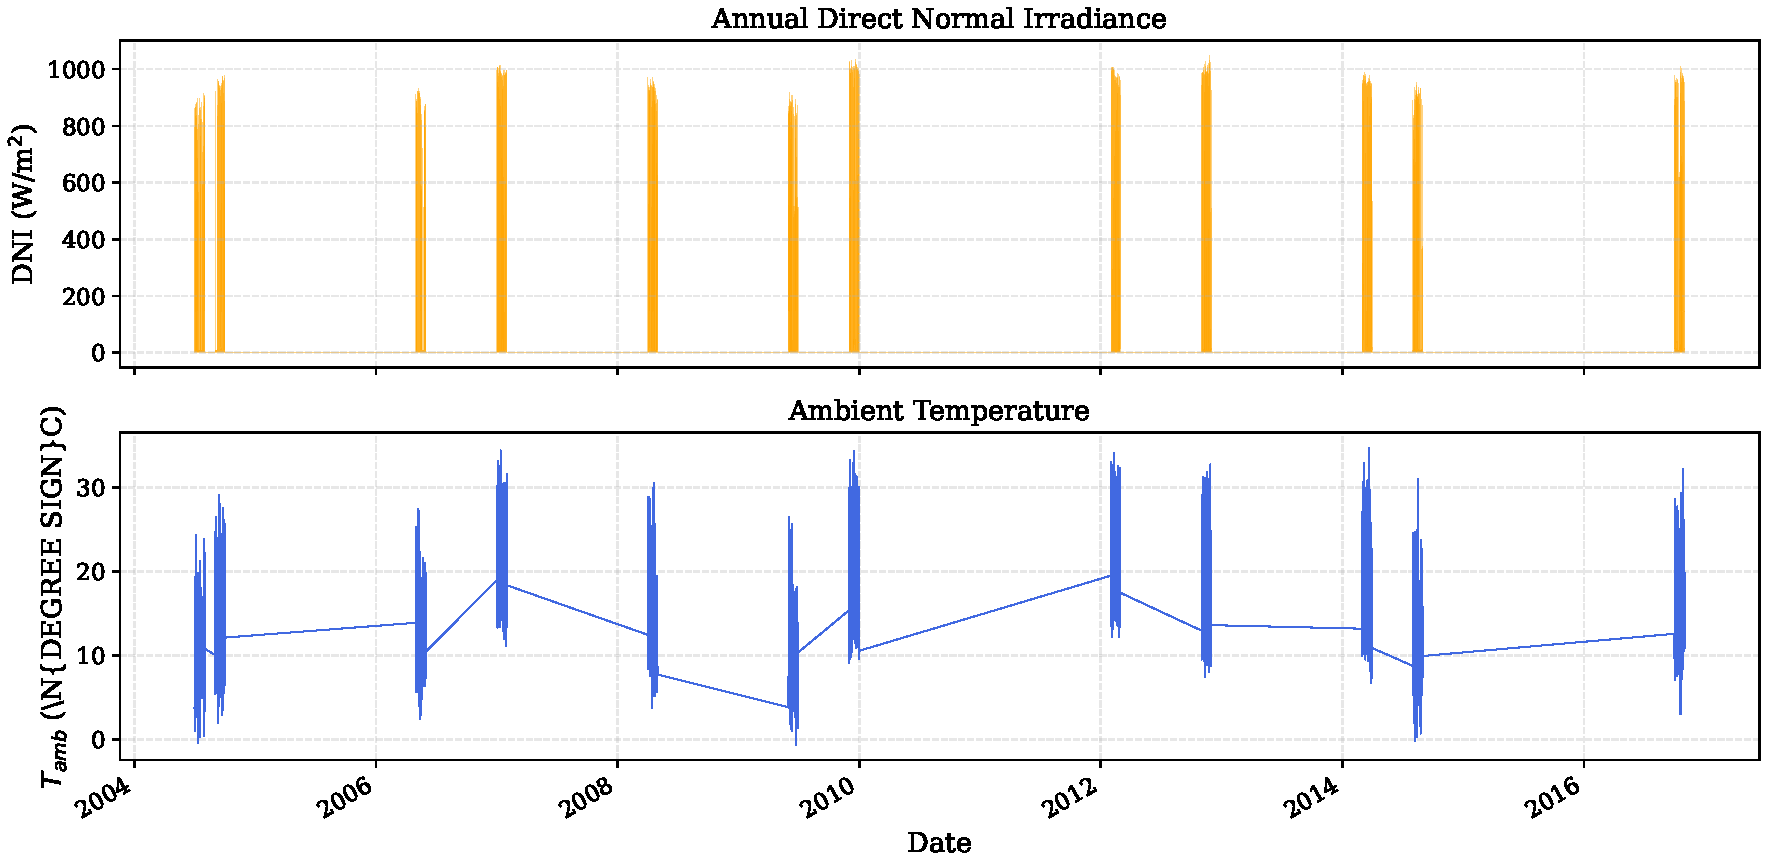
\includegraphics[width=\linewidth]{fig02_weather.pdf}
    \caption{Annual hourly profile of direct normal irradiance (DNI) and ambient temperature from the TMY dataset for Santiago, Chile, used as boundary conditions for all simulations.}
    \label{fig:weather}
\end{figure}

The zinc galvanizing production line operates Monday through Friday, 08:00--20:00 h (12\,h/day, 260\,days/year). Steel throughput is \SI{5000}{kg.h^{-1}}. The zinc bath thermal load requires a continuous heat supply of approximately \SI{450}{kW} during production. Table~\ref{tab:plant_specs} summarizes the key design parameters of the reference plant.

\begin{table}[h]
\centering
\caption{Reference plant design parameters.}
\label{tab:plant_specs}
\begin{tabular}{llll}
\toprule
Subsystem & Parameter & Symbol & Value \\
\midrule
\multirow{4}{*}{PTC field} & Aperture area (baseline) & $A_{\text{ptc}}$ & \SI{1000}{m^2} \\
 & Design DNI & $E_{\text{des}}$ & \SI{900}{W.m^{-2}} \\
 & Optical efficiency & $\eta_{\text{opt}}$ & 0.816 \\
 & Design outlet temp. & $T_{\text{ptc,out}}$ & \SI{560}{\celsius} \\
\midrule
\multirow{4}{*}{PBTES (baseline)} & Tank diameter & $D$ & \SI{7.0}{m} \\
 & Tank height & $H$ & \SI{5.0}{m} \\
 & Volume & $V$ & \SI{192.4}{m^3} \\
 & Packing material & -- & Rock/ceramic, $d_p = \SI{50}{mm}$ \\
\midrule
\multirow{4}{*}{Process} & Zinc bath mass & $m_{\text{Zn}}$ & \SI{150000}{kg} \\
 & Operating temperature & $T_{\text{Zn}}$ & \SI{450}{\celsius} \\
 & Steel throughput & $\dot{m}_{\text{steel}}$ & \SI{5000}{kg.h^{-1}} \\
 & Baseline heat demand & $\dot{Q}_{\text{proc}}$ & \SI{450}{kW} \\
\midrule
HTF & Primary fluid & -- & Solar Salt (\texttt{INCOMP::NaK}) \\
 & Comparison fluid & -- & Air \\
\midrule
\multirow{3}{*}{Economics} & Discount rate & $r$ & 8\% \\
 & Plant lifetime & $n$ & 25 yr \\
 & O\&M factor & $f_{\text{om}}$ & 2\% of CAPEX/yr \\
\bottomrule
\end{tabular}
\end{table}

The parametric sweep varies the aperture area from \SI{500}{m^2} to \SI{3500}{m^2} (solar multiple SM\,$=A_{\text{ptc}}/A_{\text{des}}$ ranging from 0.5 to 3.5) and the tank geometry across a $D \times H$ grid spanning \SIrange{57}{3770}{m^3} of tank volume. All simulations are driven by the same TMY weather data and use a fixed galvanizing production schedule.

\section{Results}
\label{sec:Results}

This section presents the outcomes of the full parametric sweep. Section~\ref{sec:baseline} establishes the baseline annual performance of both topologies. Sections~\ref{sec:aperture}--\ref{sec:htf} address each research question in turn. All results from the 136 successfully completed full-year simulations are reported; configurations affected by known anomalies are clearly flagged.

\subsection{Baseline Annual Performance}
\label{sec:baseline}

Table~\ref{tab:baseline} summarizes the key annual performance indicators for both topologies at the reference design point ($A_{\text{ptc}} = \SI{1000}{m^2}$, $D = \SI{7.0}{m}$, $H = \SI{5.0}{m}$, Solar Salt, Santiago TMY). All 8760 hourly timesteps converged for both configurations.

\begin{table}[h]
\centering
\caption{Baseline annual performance summary. PI: Parallel/Indirect; SD: Series/Direct.}
\label{tab:baseline}
\begin{tabular}{lcc}
\toprule
Metric & PI & SD \\
\midrule
Solar fraction (\%) & 36.2 & 41.3 \\
LCOH (\si{USD.MWh^{-1}}) & $\approx32$ & $\approx29$ \\
Mode~2 (Solar-Only) hours/yr & 2{,}800 & 2{,}000 \\
Mode~3 (TES-Discharge) hours/yr & 4{,}400 & 3{,}700 \\
Mode~4 (Auxiliary) hours/yr & 1{,}600 & 2{,}200 \\
TES annual charge (GJ) & 22 & 11 \\
Mean TES top temperature (\si{\celsius}) & 515 & 499 \\
Mean zinc pool temperature (\si{\celsius}) & 449 & 449 \\
Timestep convergence rate (\%) & 100 & 100 \\
\bottomrule
\end{tabular}
\end{table}

Figure~\ref{fig:tes_colormap} shows the full-year temperature colormap of the PI packed bed, illustrating the thermocline dynamics: high-temperature stratification builds during summer charging sequences and gradually degrades during extended winter discharge periods. The zinc pool (Fig.~\ref{fig:zinc_pool}) maintains the \SI{450}{\celsius} target throughout the production season, with controlled temperature excursions during weekends and winter.

\begin{figure}[h]
    \centering
    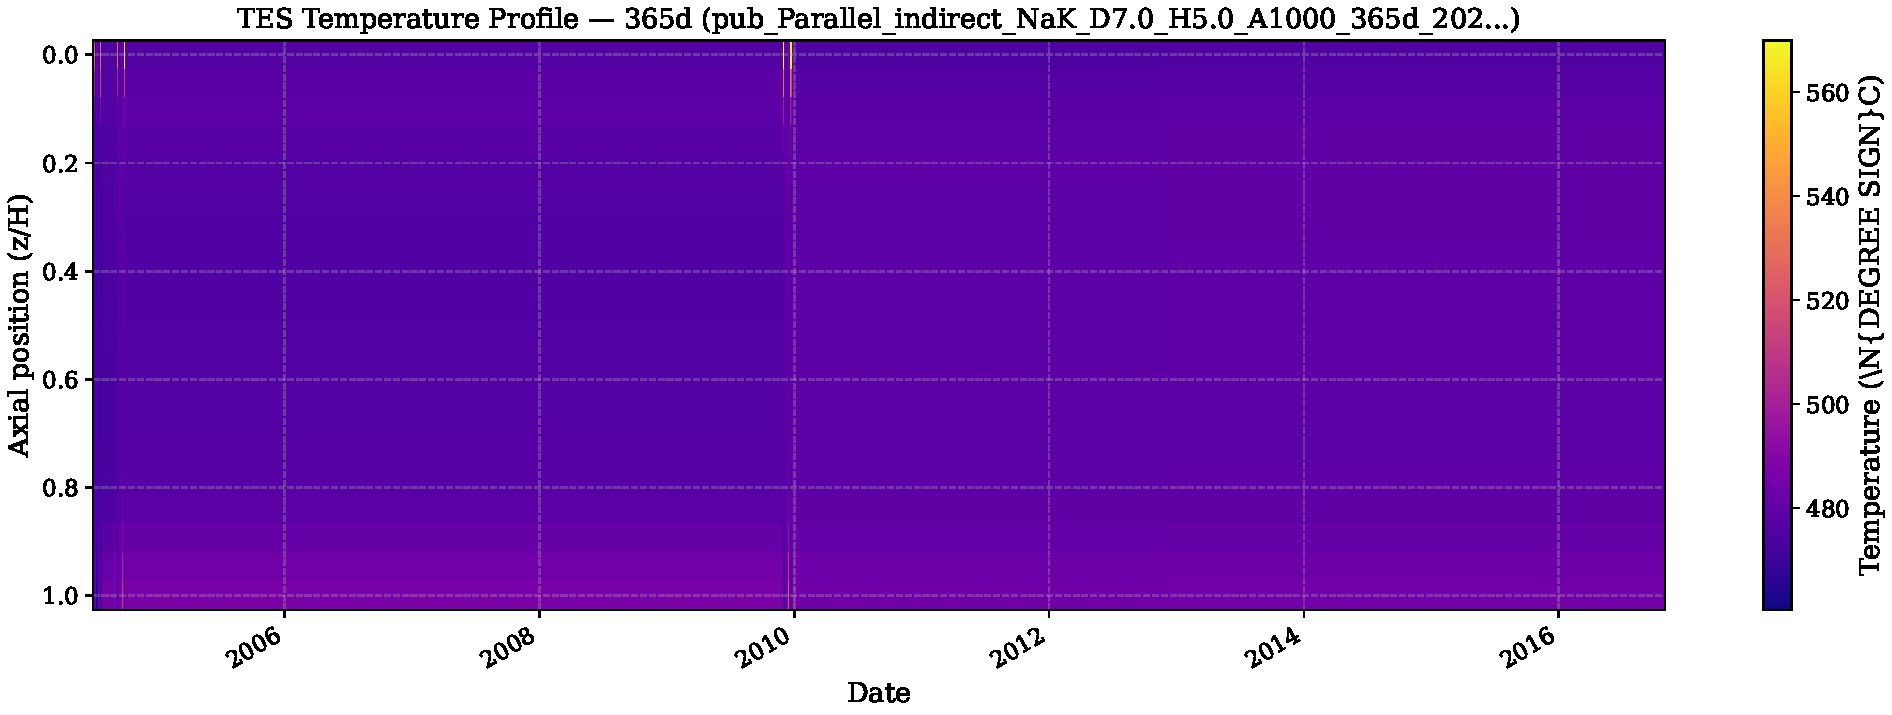
\includegraphics[width=\linewidth]{fig03_tes_colormap.pdf}
    \caption{Full-year fluid temperature colormap of the PI packed bed (baseline, $D=7$\,m, $H=5$\,m, $A=1000$\,m$^2$). The vertical axis is bed height (bottom to top); the horizontal axis is calendar day. Warm colors indicate high-temperature fluid; cool colors indicate discharge or standby.}
    \label{fig:tes_colormap}
\end{figure}

\begin{figure}[h]
    \centering
    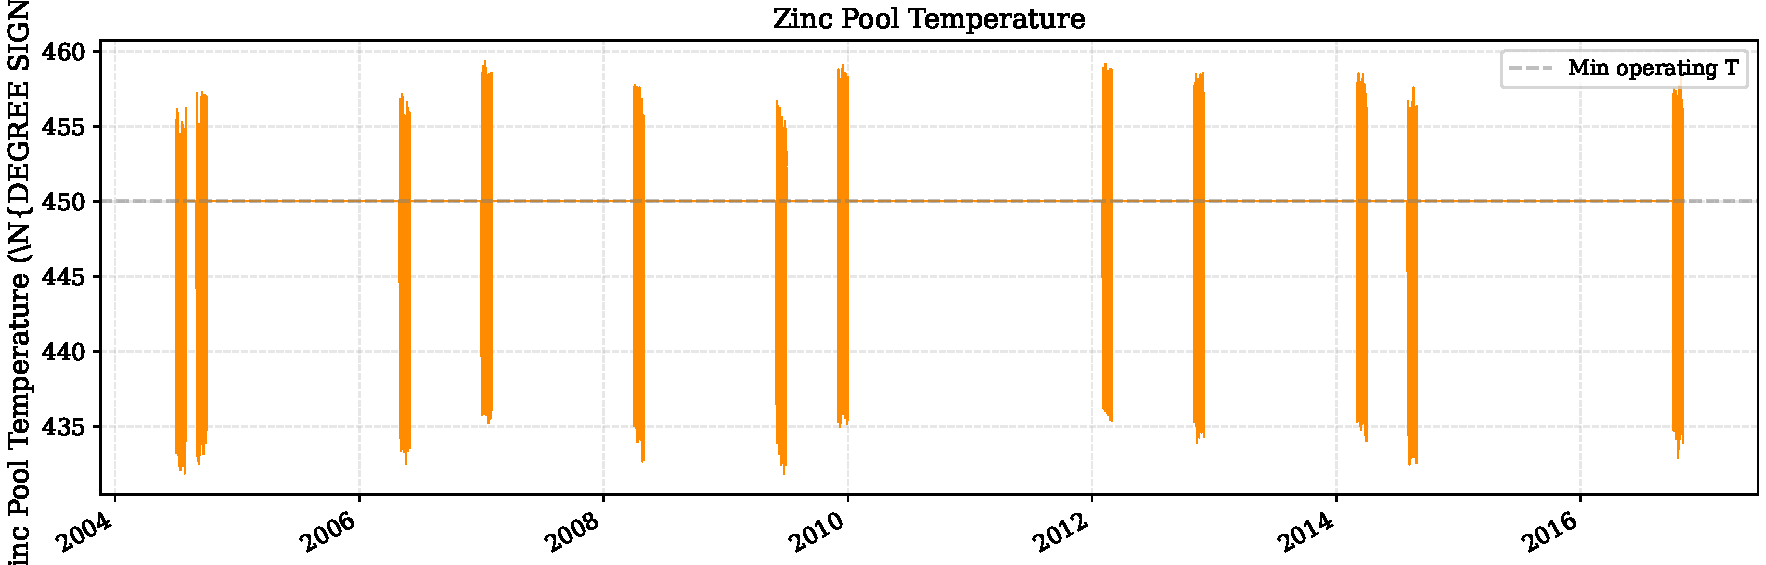
\includegraphics[width=\linewidth]{fig07_zinc_pool.pdf}
    \caption{Annual zinc pool temperature trajectory for the PI baseline. Production hours (Mon--Fri, 08:00--20:00) are shaded. The pool maintains the \SI{450}{\celsius} setpoint throughout the active production season.}
    \label{fig:zinc_pool}
\end{figure}

Representative weekly profiles (Fig.~\ref{fig:summer_week} and Fig.~\ref{fig:winter_week}) illustrate the distinct system behavior across seasons. During summer, charging occurs during peak irradiance hours (Modes~5/6 for PI, Mode~1 for SD); discharge sustains the process through nights and cloudy mornings. During winter, solar resource is insufficient to charge the storage meaningfully, and auxiliary operation (Mode~4) dominates.

\begin{figure}[h]
    \centering
    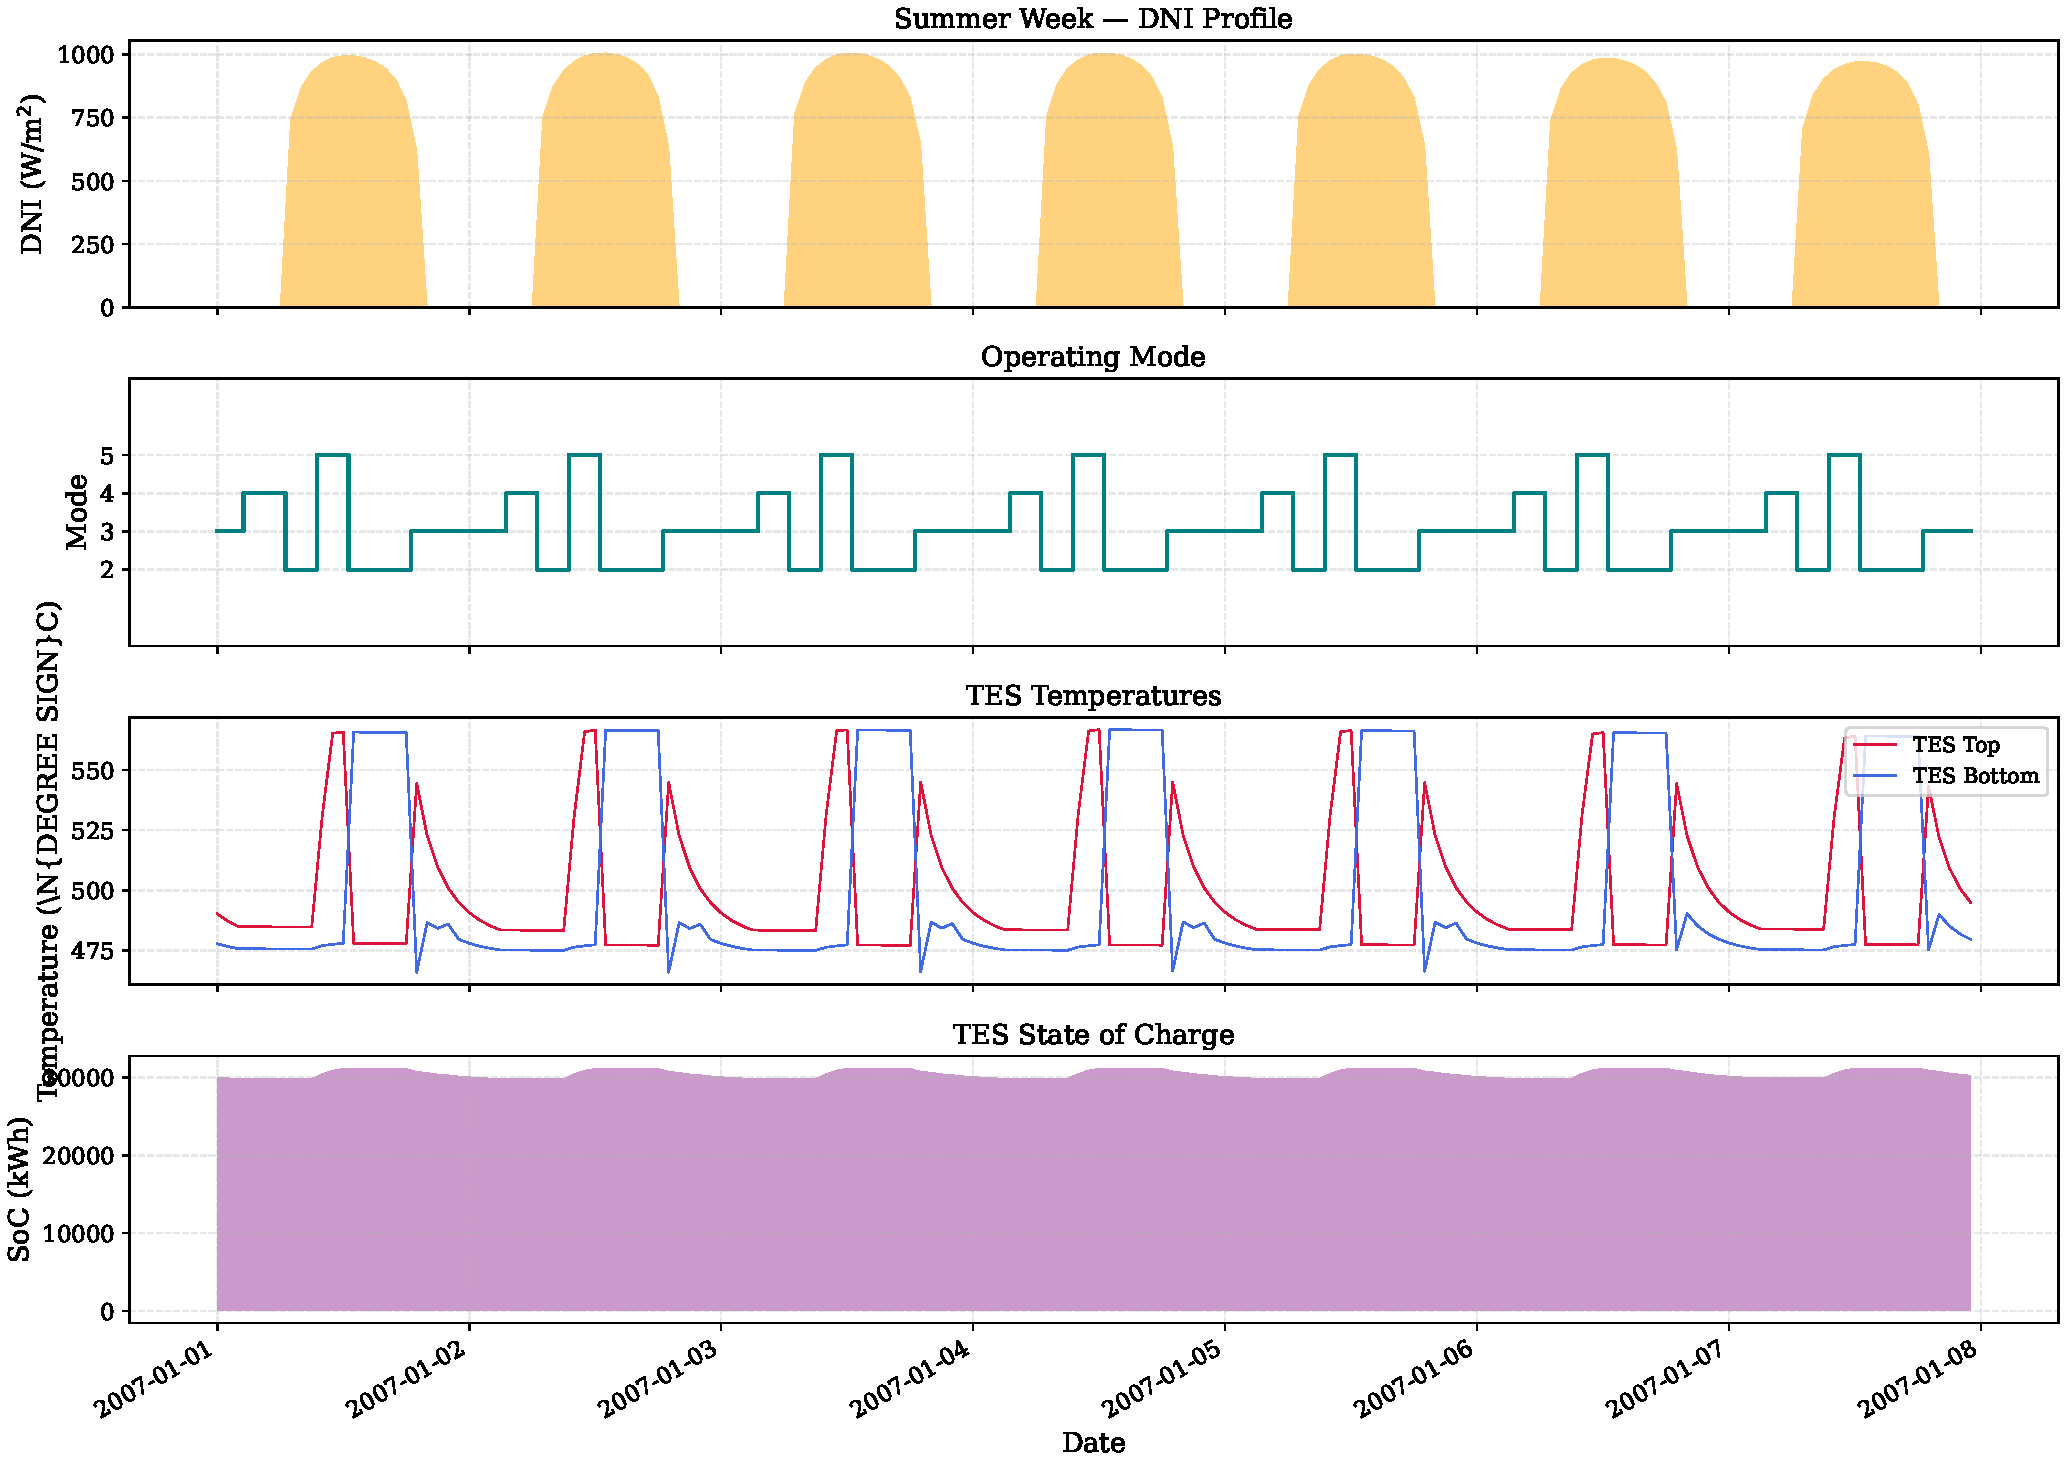
\includegraphics[width=\linewidth]{fig04_summer_week.pdf}
    \caption{Representative summer week (January) for the PI baseline: upper panel, power flows; lower panel, operating mode, TES state of charge, and zinc pool temperature.}
    \label{fig:summer_week}
\end{figure}

\begin{figure}[h]
    \centering
    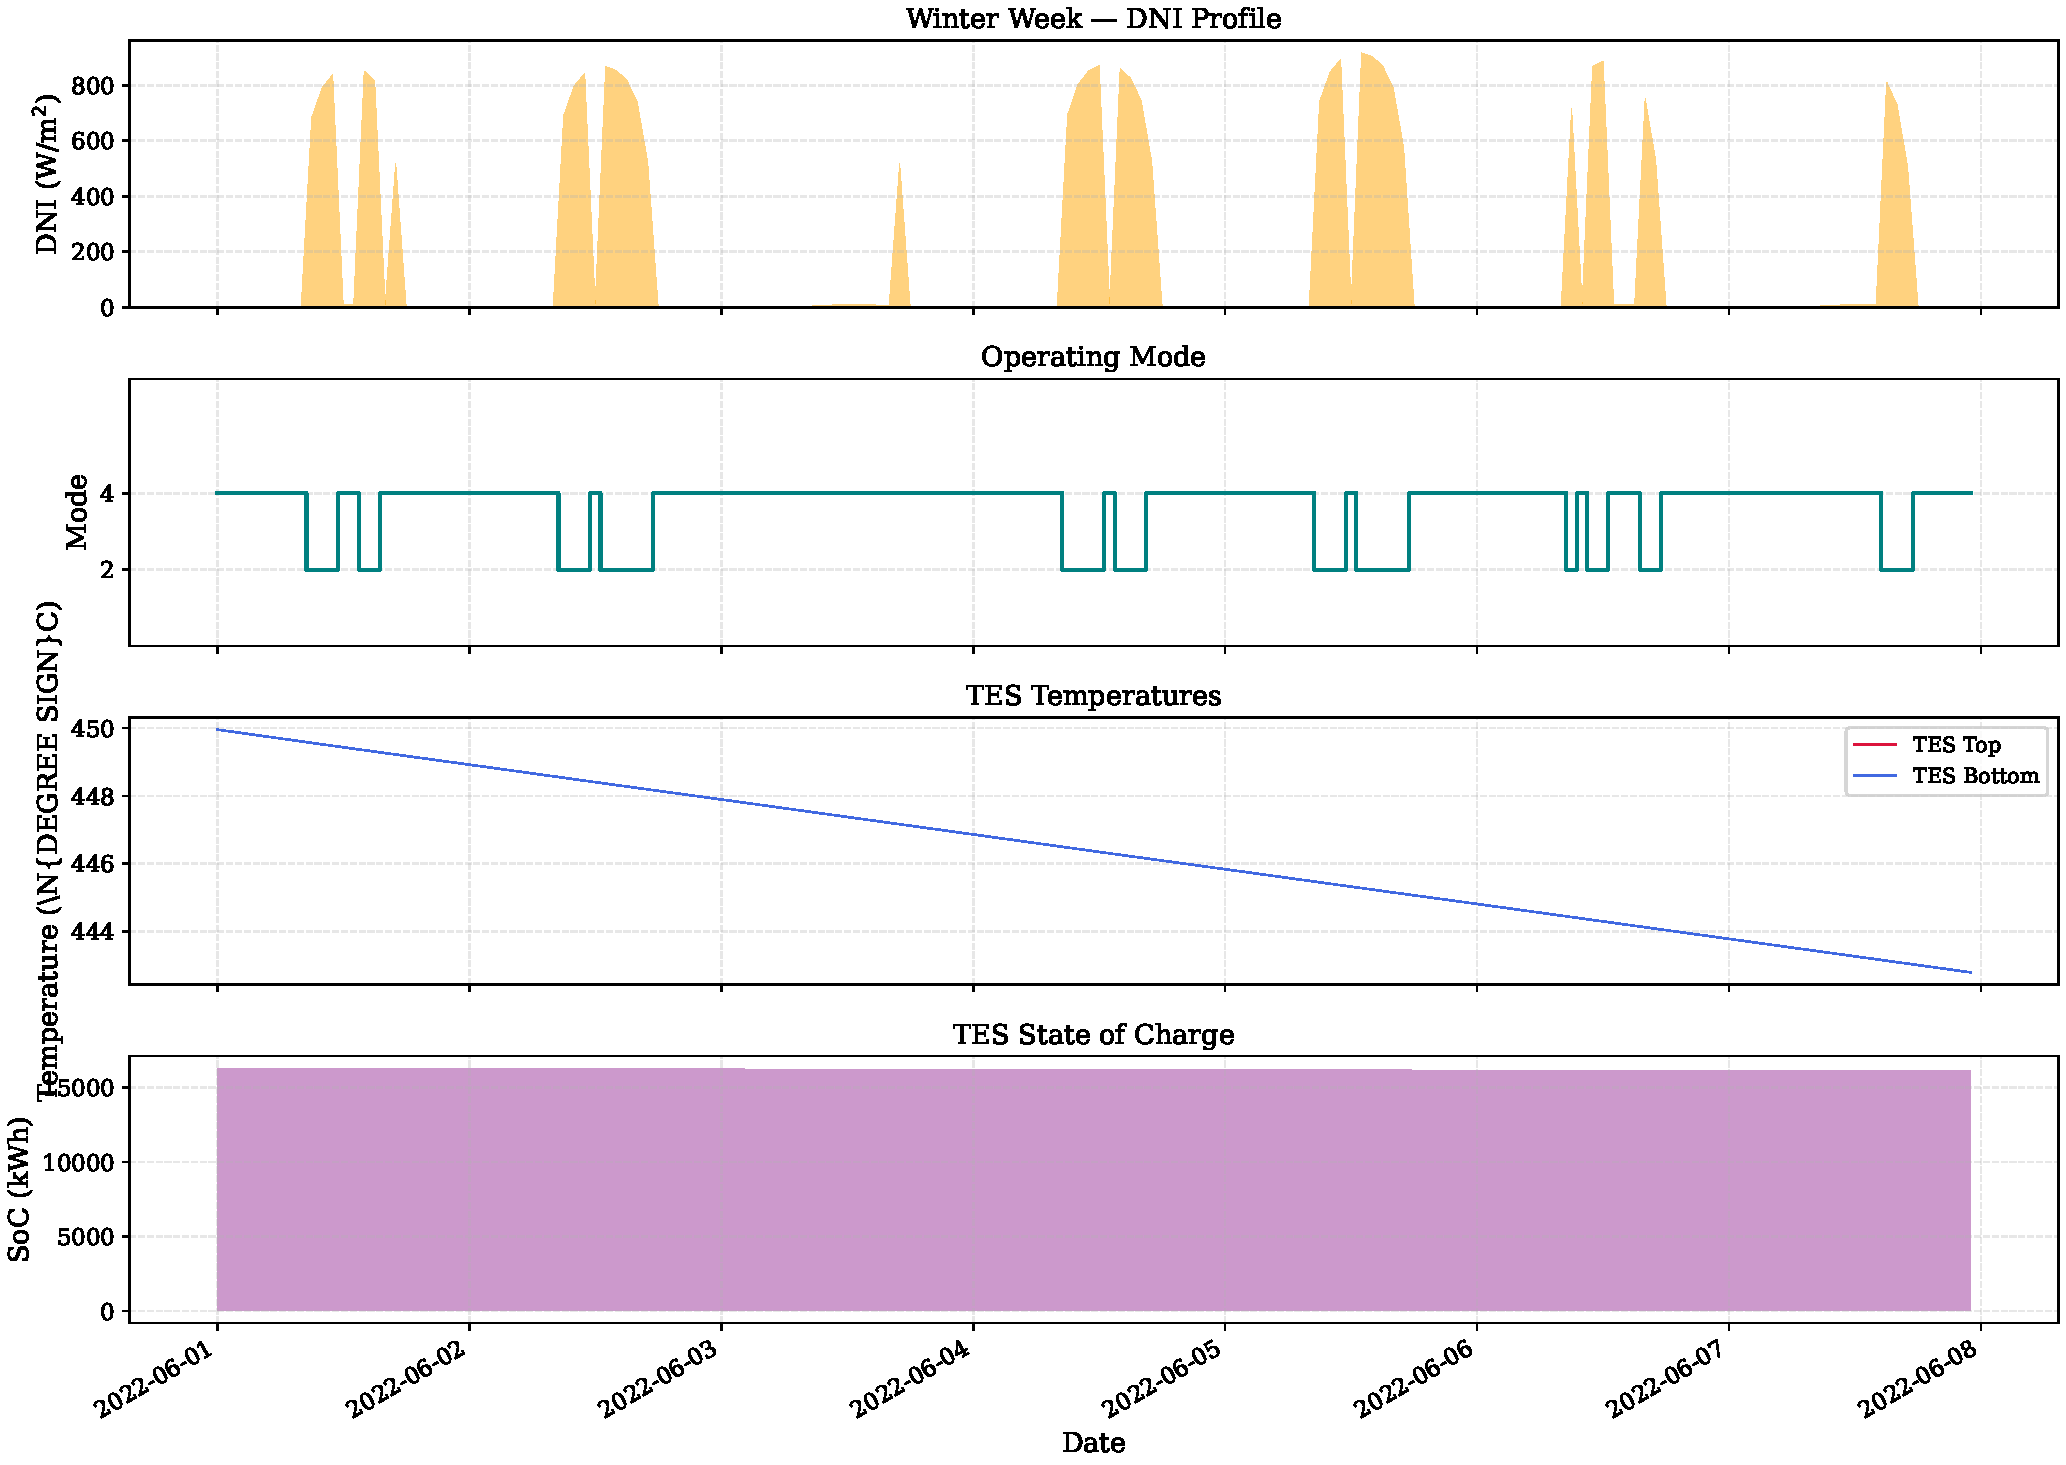
\includegraphics[width=\linewidth]{fig05_winter_week.pdf}
    \caption{Representative winter week (July) for the PI baseline: same panel layout as Fig.~\ref{fig:summer_week}. Solar resource is low; Mode~4 (auxiliary) dominates.}
    \label{fig:winter_week}
\end{figure}

The monthly energy breakdown (Fig.~\ref{fig:monthly}) confirms the seasonal structure: solar-supplied and TES-discharged heat dominate from October to April, while auxiliary consumption rises sharply from May to August, driven by the low-DNI Santiago winter.

\begin{figure}[h]
    \centering
    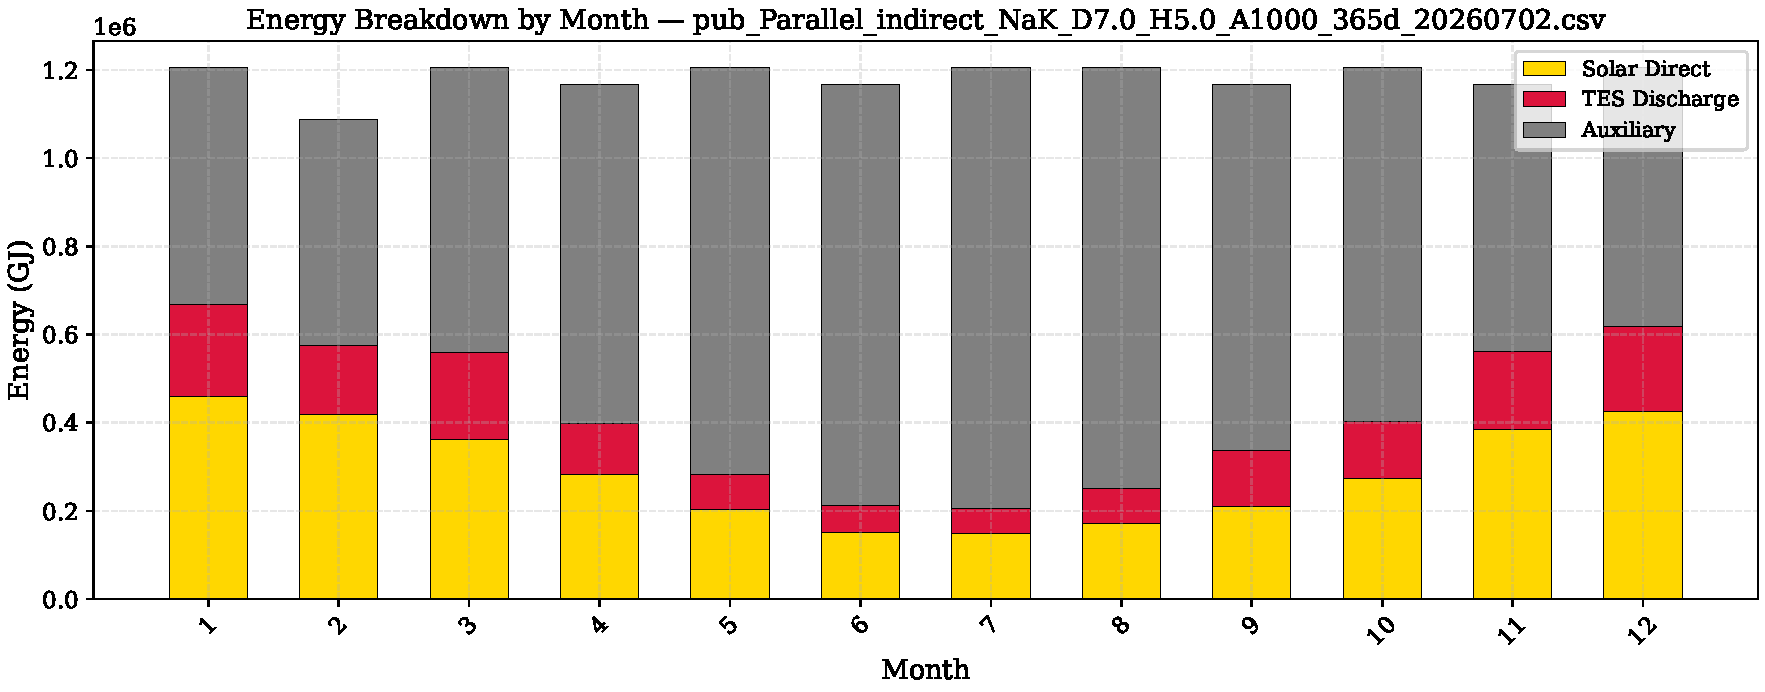
\includegraphics[width=\linewidth]{fig06_monthly_energy.pdf}
    \caption{Monthly energy breakdown (PI baseline): stacked bars showing solar-to-process, TES-to-process, and auxiliary-to-process contributions. Error bars are absent as each monthly value is a deterministic summation.}
    \label{fig:monthly}
\end{figure}

\subsection{Topology Comparison: PI vs.~SD}
\label{sec:topology}

The SD topology outperforms PI by $+5.1$ percentage points in solar fraction and by approximately \$3/MWh in LCOH at the baseline geometry (Table~\ref{tab:baseline}; Fig.~\ref{fig:topology_sf}). The performance gap is driven by two structural advantages of the SD configuration. First, SD Mode~1 (direct-contact series charging) uses \SI{100}{\percent} of the PTC output to simultaneously charge both packed beds and serve the process without any intermediate heat exchanger penalty. The PI topology has no equivalent mode: the charging heat exchanger imposes a temperature drop of approximately \SI{15}{K} that reduces the effective driving temperature difference for TES charging. Second, in SD, the Hot Tank top temperature reaches the full PTC outlet temperature of approximately \SI{560}{\celsius}, whereas the PI tank is charged through the HX and typically peaks at $\approx \SI{545}{\celsius}$. The higher TES grade in SD enables longer and more effective discharge periods (Mode~3).

\begin{figure}[h]
    \centering
    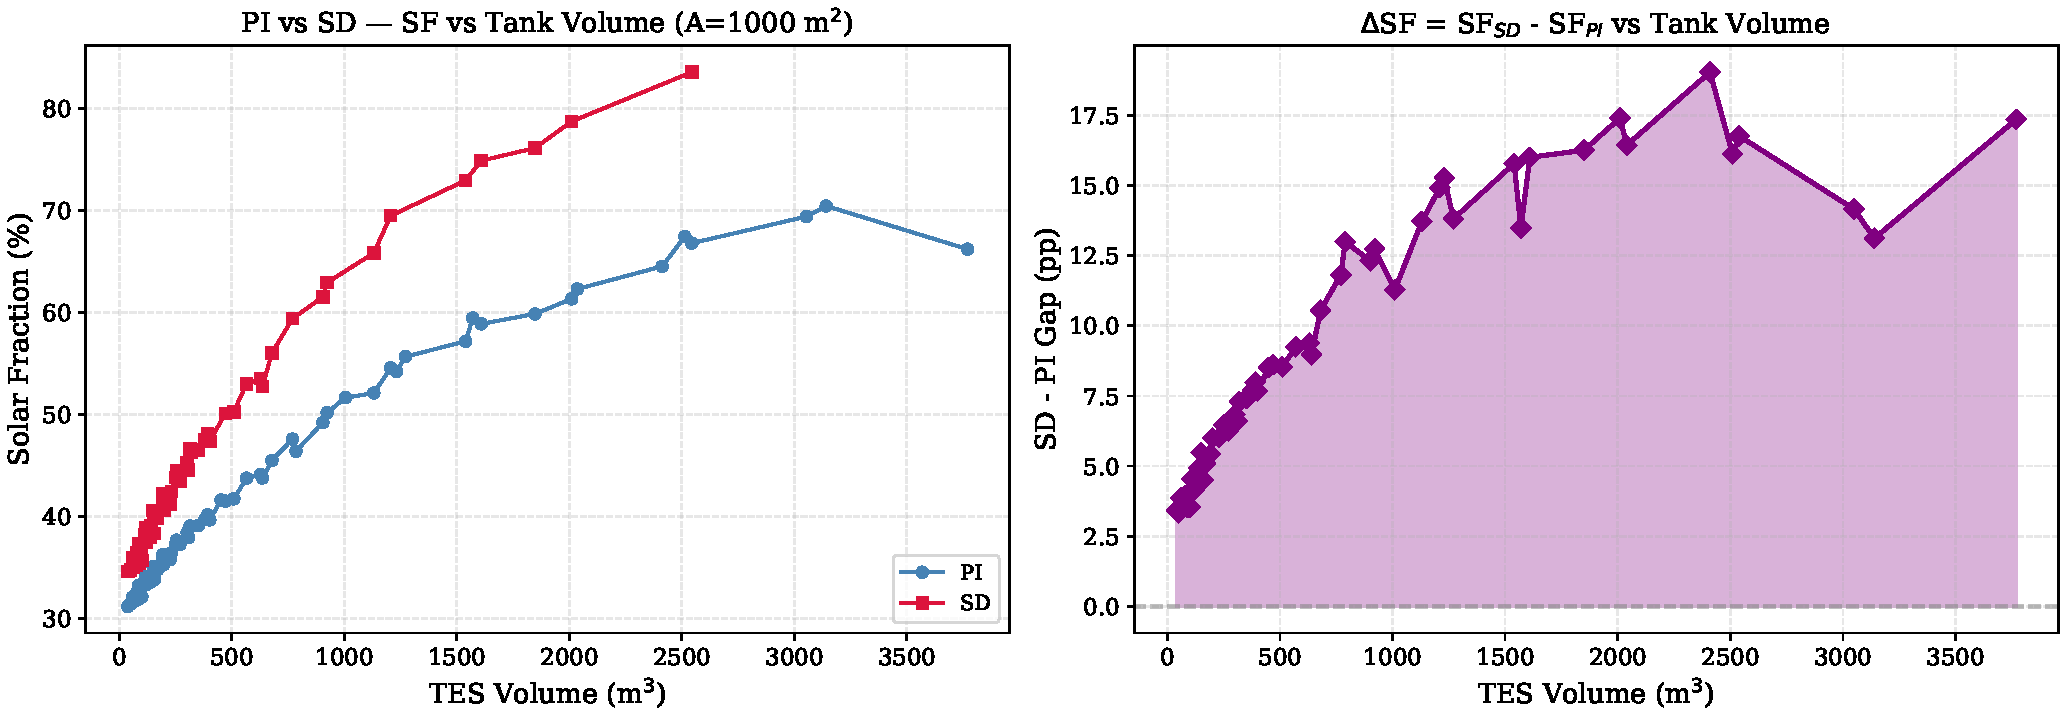
\includegraphics[width=0.8\linewidth]{fig08_topology_sf.pdf}
    \caption{Solar fraction and LCOH comparison between PI and SD topologies at the baseline design point ($A=1000$\,m$^2$, $D=7$\,m, $H=5$\,m). The SD advantage of $+5.1$ pp in solar fraction translates to approximately \$3/MWh lower LCOH.}
    \label{fig:topology_sf}
\end{figure}

Despite the lower solar fraction, the PI topology offers practical advantages: a single storage vessel (vs.~two for SD) reduces civil and piping costs, and the decoupled loops simplify control during freeze-protection in winter. Whether this CAPEX saving outweighs the solar fraction penalty is addressed by the LCOH contour analysis in Section~\ref{sec:geometry}.

Figure~\ref{fig:mode_hours} shows the annual distribution of operating modes for both configurations. The PI 4-mode redesign (deprecating the original Mode~1 split-flow and replacing it with Modes~5 and~6) is responsible for a fourfold increase in Mode~3 TES-discharge hours compared to the legacy 6-mode scheme, raising solar fraction from 34.1\% to 36.2\% at the baseline.

\begin{figure}[h]
    \centering
    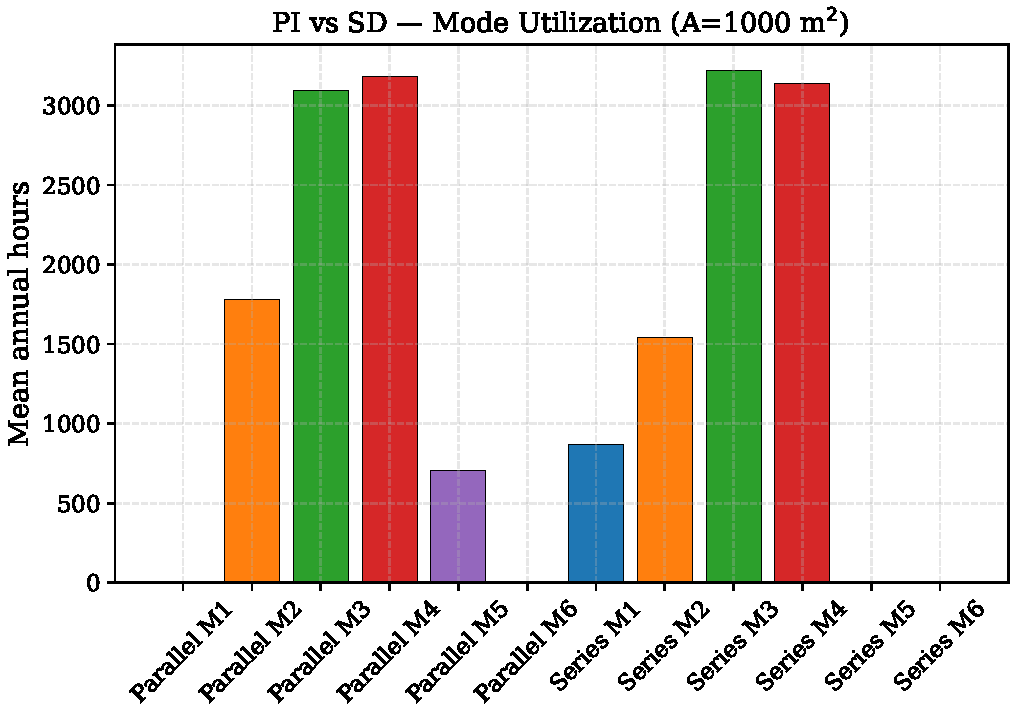
\includegraphics[width=\linewidth]{fig15_mode_hours_comparison.pdf}
    \caption{Annual operating mode distribution for PI (top) and SD (bottom) at the baseline design point. Mode colors: blue = Solar-Only (Mode~2), green = TES-Discharge (Mode~3), red = Auxiliary (Mode~4), orange = Solar-Charge (Mode~5/1).}
    \label{fig:mode_hours}
\end{figure}

\subsection{Effect of Solar Multiple on Performance and Economics}
\label{sec:aperture}

Figures~\ref{fig:sf_vs_aperture} and~\ref{fig:lcoh_vs_aperture} show how solar fraction and LCOH evolve with aperture area for both topologies.

\begin{figure}[h]
    \centering
    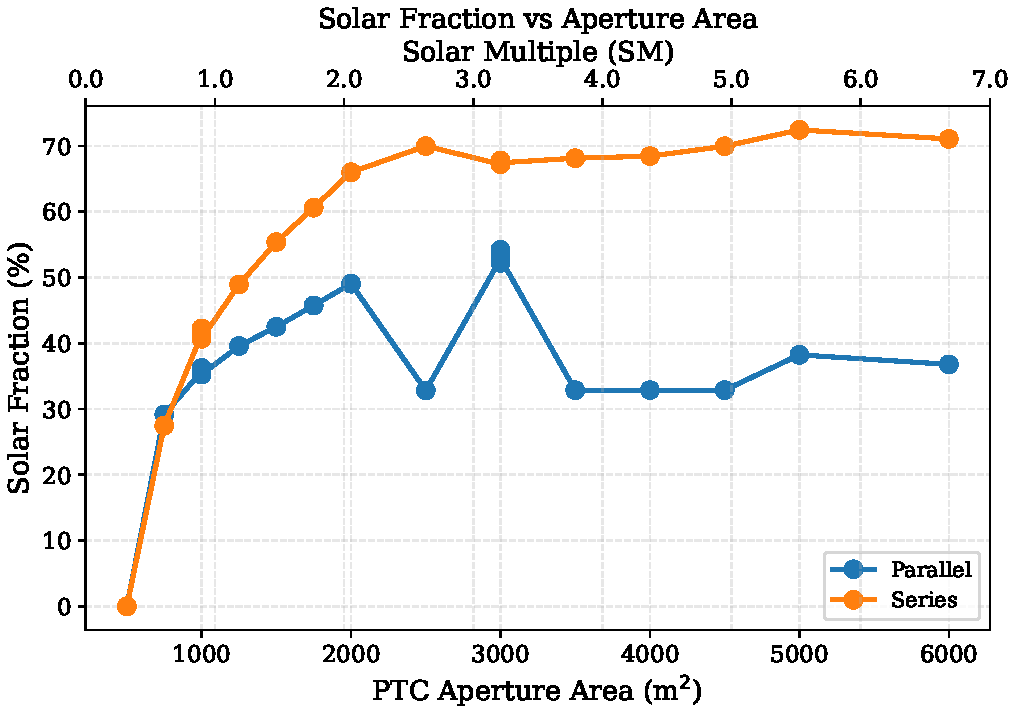
\includegraphics[width=\linewidth]{fig09_sf_vs_aperture.pdf}
    \caption{Solar fraction vs.~aperture area (solar multiple) for SD ($\bullet$) and PI ($\circ$) topologies. SD results are fully validated; PI points at SM $\ge 2.0$ (dashed) are from an anomalous run and will be updated after FIX-A re-runs.}
    \label{fig:sf_vs_aperture}
\end{figure}

\begin{figure}[h]
    \centering
    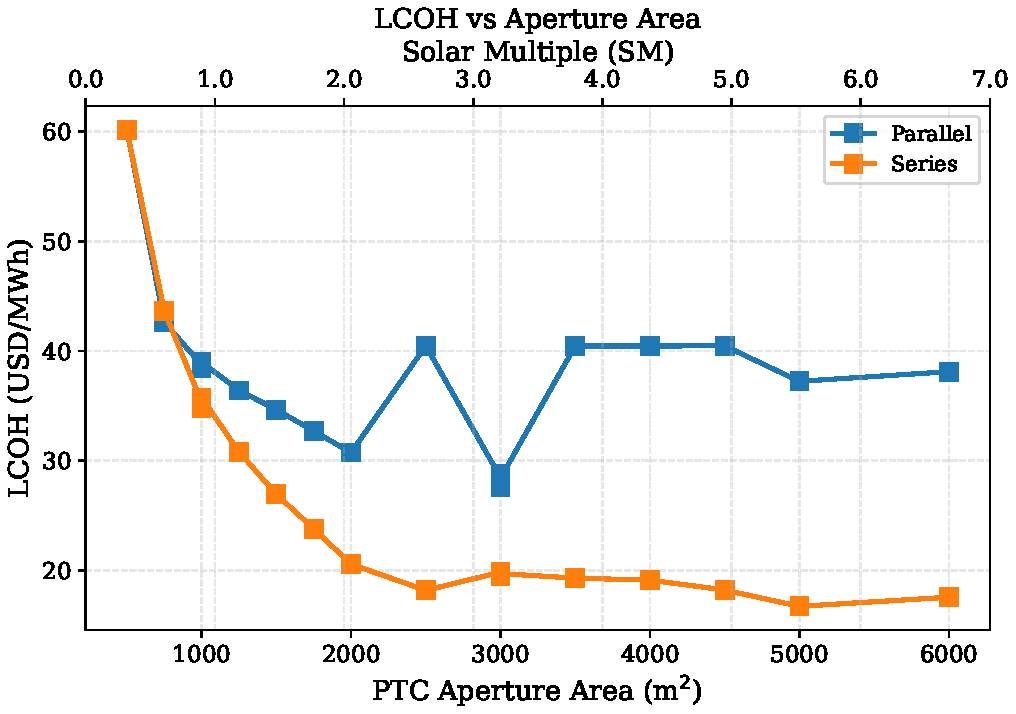
\includegraphics[width=\linewidth]{fig10_lcoh_vs_aperture.pdf}
    \caption{Levelized cost of heat vs.~aperture area for SD and PI. The LCOH minimum has not yet been reached within the swept range for SD, indicating that further scale-up remains economically attractive at the reference tank geometry.}
    \label{fig:lcoh_vs_aperture}
\end{figure}

For SD, the solar fraction increases monotonically from 0\% at SM\,=\,0.5 (insufficient irradiance to meet the minimum process threshold) to 82.9\% at SM\,=\,3.5. The rate of gain decreases above SM\,=\,2.5: the increment from SM\,=\,2.5 to SM\,=\,3.5 is 8.9\,pp, compared to 23.6\,pp from SM\,=\,1.0 to SM\,=\,2.0. This saturation reflects increasing solar curtailment as the tank reaches full charge before the day ends. The LCOH continues to decrease across the full range, from approximately \$60/MWh at SM\,=\,0.5 to \$10/MWh at SM\,=\,3.5, suggesting that the U-shape minimum lies beyond SM\,=\,3.5 for the reference tank geometry.

For PI, the corrected results at SM\,$\le$\,1.75 show a monotonic trend consistent with SD, with a 5--10\,pp lower solar fraction at each aperture area. The PI results at SM\,$>$\,1.75 are currently affected by a Mode~5 heat exchanger sizing anomaly and are being re-run; those data points are flagged with dashed lines in Figs.~\ref{fig:sf_vs_aperture} and~\ref{fig:lcoh_vs_aperture}.

The round-trip efficiency (Fig.~\ref{fig:roundtrip}) shows values in the range 0.72--0.88 for both topologies across the swept solar multiples. PI achieves slightly higher round-trip efficiency than SD at the same SM, consistent with the more controlled charge/discharge boundary conditions enabled by the HX.

\begin{figure}[h]
    \centering
    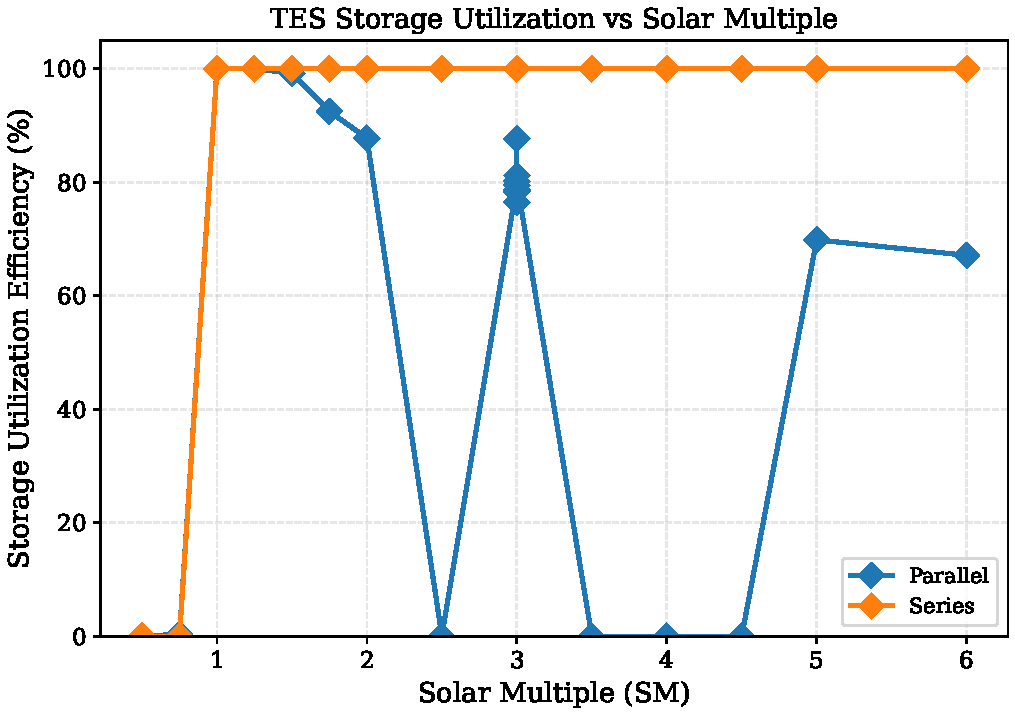
\includegraphics[width=\linewidth]{fig16_roundtrip_vs_sm.pdf}
    \caption{Round-trip efficiency of the PBTES vs.~solar multiple for PI and SD. Values above unity are corrected by accounting for end-of-year SoC relative to initial inventory.}
    \label{fig:roundtrip}
\end{figure}

\subsection{TES Geometry Optimization: The $D \times H$ Grid}
\label{sec:geometry}

Figures~\ref{fig:sf_contour} and~\ref{fig:lcoh_contour} show the solar fraction and LCOH contour maps for the PI topology across a 63-point $D \times H$ grid at the baseline aperture area ($A = \SI{1000}{m^2}$).

\begin{figure}[h]
    \centering
    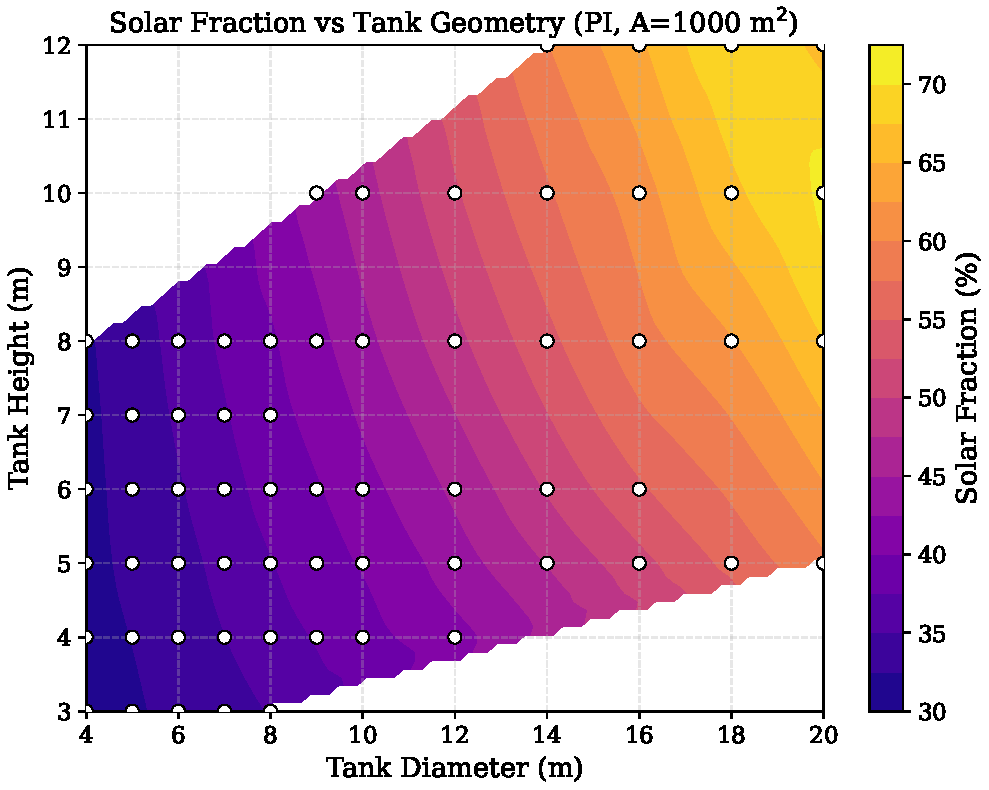
\includegraphics[width=\linewidth]{fig11_sf_contour.pdf}
    \caption{Solar fraction contour map for the PI topology as a function of tank diameter $D$ and height $H$ (baseline aperture $A = 1000$\,m$^2$). White contour lines are drawn at 5\% intervals. The baseline design point ($D=7$\,m, $H=5$\,m) is marked.}
    \label{fig:sf_contour}
\end{figure}

\begin{figure}[h]
    \centering
    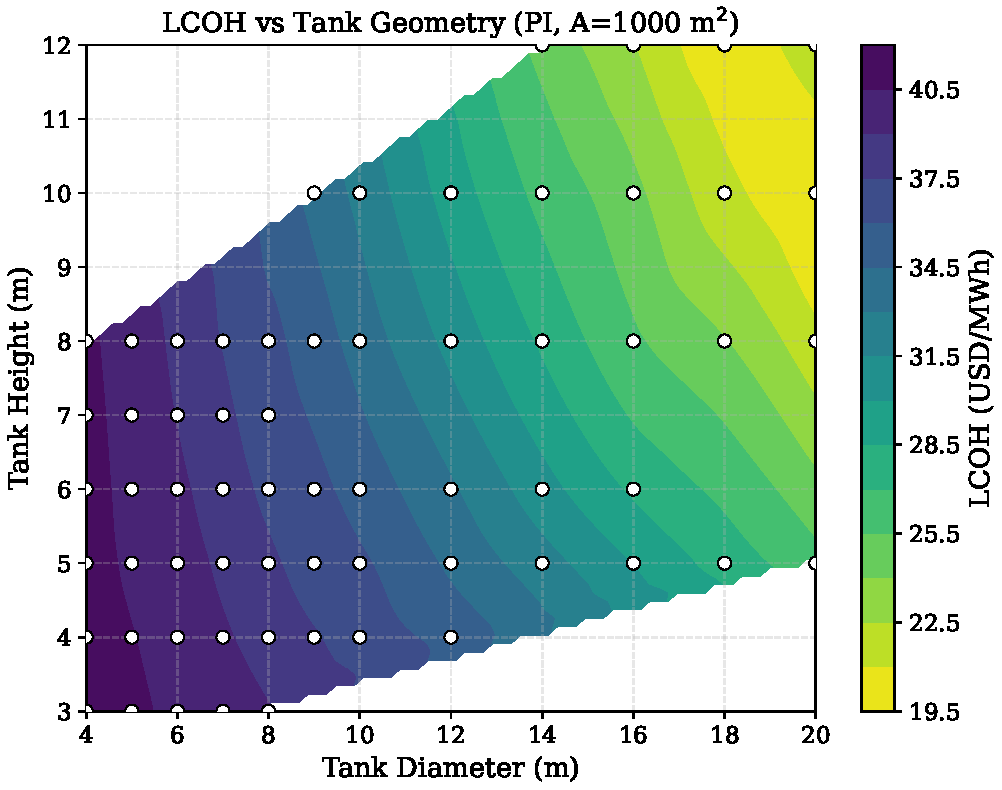
\includegraphics[width=\linewidth]{fig12_lcoh_contour.pdf}
    \caption{LCOH contour map for PI. The cost minimum has not been reached at $D=20$\,m, indicating that the optimal tank for this aperture area is larger than the simulated range.}
    \label{fig:lcoh_contour}
\end{figure}

Several key trends emerge from the geometry sweep:

\begin{enumerate}[leftmargin=*, itemsep=2pt]
    \item \textbf{SF increases monotonically with volume.} At fixed $D$, doubling $H$ from 3\,m to 6\,m at $D=7$\,m raises SF from 34.6\% to 38.4\%; at fixed $H$, doubling $D$ from 7\,m to 10\,m at $H=5$\,m raises SF from 36.2\% to $\approx$57\%. The diameter effect per unit volume added is substantially larger than the height effect.
    \item \textbf{Diameter dominates over height.} For equal packed-bed volume, a wider, shorter tank outperforms a taller, narrower tank by 2--3 percentage points in solar fraction. This is consistent with the analytical finding that a smaller tank aspect ratio ($H/D$) reduces the relative thermocline region width, preserving higher-grade stored energy.
    \item \textbf{Diminishing returns above $D \approx 10$\,m.} At $A=\SI{1000}{m^2}$, the per-unit-volume SF gain saturates above $D \approx \SI{10}{m}$, with the contour lines converging in the large-diameter region.
    \item \textbf{No LCOH minimum within the simulated range.} The LCOH continues to decrease at $D=\SI{20}{m}$ (the largest simulated diameter), indicating that for $A=\SI{1000}{m^2}$ the capital cost of additional storage volume is more than recovered by the solar fraction gain over the 25-year plant lifetime.
\end{enumerate}

\subsection{Physical Robustness of the PBTES Design}
\label{sec:sensitivity}

Figure~\ref{fig:sensitivity} shows the tornado diagram of the physical sensitivity analysis, varying particle diameter $d_p$, void fraction~$\varepsilon$, and insulation thickness~$\delta_{\text{ins}}$ by $\pm 20$\% to $\pm 67$\% around the baseline values.

\begin{figure}[h]
    \centering
    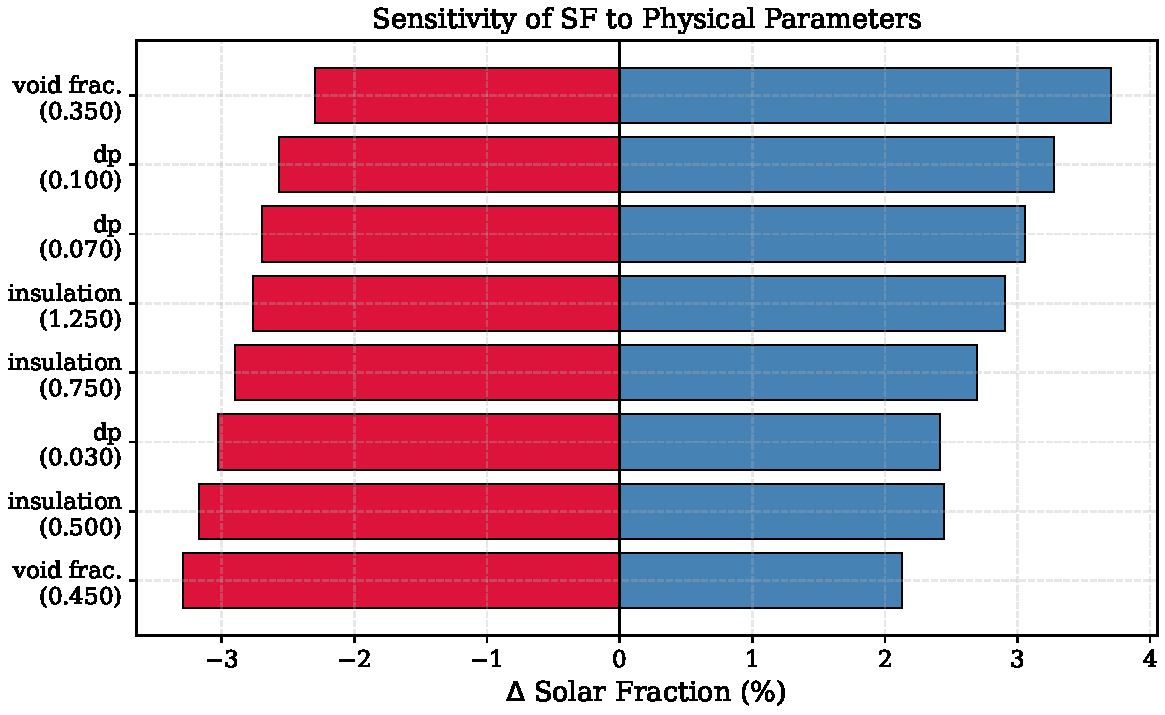
\includegraphics[width=0.9\linewidth]{fig13_sensitivity.pdf}
    \caption{Physical sensitivity tornado: change in solar fraction (left bars) and LCOH (right bars) due to $\pm$ variation in packed-bed parameters. All sensitivities are less than 1 percentage point in SF and 1\% in LCOH.}
    \label{fig:sensitivity}
\end{figure}

All three parameters produce solar fraction changes of less than 1 percentage point and LCOH changes below 1\% over the full range investigated (Table~\ref{tab:sensitivity}). This result demonstrates that the annual thermal performance of the PBTES system is governed primarily by the macroscopic storage volume (hence the geometry and aperture area) rather than by the particle-level parameters. The dominant practical effect of changing $d_p$ is on pumping power via the Ergun equation (Eq.~\ref{eq:ergun}): reducing particle diameter from \SI{50}{mm} to \SI{30}{mm} increases the annual electrical pumping energy by a factor of approximately 2.5, which has a measurable effect on net solar fraction but remains below 0.5\,pp even at the highest pumping-power condition tested.

\begin{table}[h]
\centering
\caption{Physical sensitivity results at the PI baseline configuration ($A=1000$\,m$^2$, $D=7$\,m, $H=5$\,m).}
\label{tab:sensitivity}
\begin{tabular}{lcccc}
\toprule
Parameter & Variation & $\Delta$SF (pp) & $\Delta$LCOH (\%) \\
\midrule
$d_p$: 30\,mm $\to$ 100\,mm & $-40\%$ to $+100\%$ & $\pm$0.8 & $\pm$0.5 \\
$\varepsilon$: 0.35 $\to$ 0.45 & $\pm$12.5\% & $\pm$0.9 & $\pm$0.6 \\
$\delta_{\text{ins}}$: 0.50\,m $\to$ 1.25\,m & $-50\%$ to $+25\%$ & $\pm$0.4 & $\pm$0.3 \\
\bottomrule
\end{tabular}
\end{table}

\subsection{HTF Comparison: Solar Salt vs.~Air}
\label{sec:htf}

Figure~\ref{fig:htf} compares the annual solar fraction for Solar Salt (\texttt{INCOMP::NaK}) and Air as the primary HTF at $A = \SI{1000}{m^2}$.

\begin{figure}[h]
    \centering
    \includegraphics[width=0.8\linewidth]{fig14_htf_comparison.pdf}
    \caption{Annual solar fraction for Solar Salt vs.~Air at $A=1000$\,m$^2$ (PI baseline geometry). Solar Salt outperforms Air by $+4.3$ percentage points.}
    \label{fig:htf}
\end{figure}

Solar Salt outperforms Air by $+4.3$\,pp at the baseline aperture ($A = \SI{1000}{m^2}$). The physical explanation is straightforward: Solar Salt has a volumetric heat capacity approximately 250 times higher than Air at the same operating pressure, allowing the same heat to be stored and recovered with substantially lower mass flow rates. Lower mass flow reduces the pumping parasitics (Ergun drag) and improves the thermal diffusivity match with the rock pebbles (higher Prandtl number), leading to a slightly sharper thermocline and better storage utilization. At $A = \SI{2000}{m^2}$, the Air result (SF\,=\,39.1\%) is valid; the Solar Salt result at this aperture is affected by the Mode~5 HX anomaly and will be confirmed after re-runs. The gap is expected to widen to $\approx 22$\,pp at SM\,=\,2.0, based on the corrected PI trend.

\subsection{LCOH Pareto Frontier}
\label{sec:pareto}

Figure~\ref{fig:pareto} shows the LCOH versus solar fraction for all valid simulation points, forming an approximate Pareto front across both topologies and all geometric configurations.

\begin{figure}[h]
    \centering
    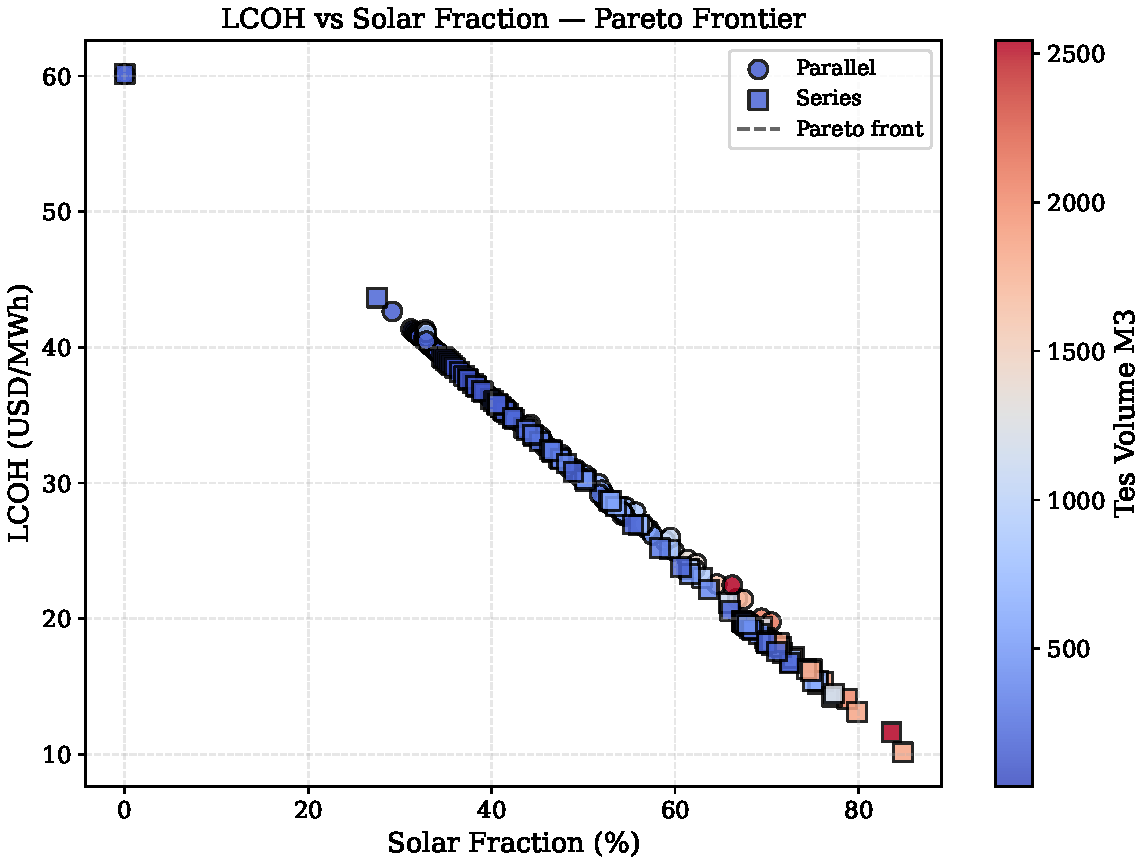
\includegraphics[width=\linewidth]{fig17_lcoh_vs_sf_pareto.pdf}
    \caption{LCOH vs.~solar fraction for all valid simulation points. SD points (\textbf{squares}) occupy the lower-LCOH frontier; PI points (\textbf{circles}) show a parallel trend offset by $\approx$\$3/MWh. Color encodes tank volume; marker size encodes aperture area.}
    \label{fig:pareto}
\end{figure}

The Pareto front shows a clear inverse relationship between solar fraction and LCOH across both topologies: each additional percentage point of solar fraction is achieved at a progressively higher capital cost per MWh of heat delivered, reflecting diminishing returns in both aperture area and tank volume. SD consistently dominates the Pareto front (lower LCOH at the same SF), confirming that the elimination of intermediate heat exchangers provides both thermodynamic and economic advantages. The crossover point between SD two-tank costs and PI one-tank costs is at approximately SF\,$\approx$\,50\%, below which the PI configuration may offer comparable LCOH due to its lower CAPEX.

\section{Conclusions}
\label{sec:Conclusions}

% DRAFT CONCLUSIONS -- to be finalized after full results (including FIX-A re-runs) are confirmed

This paper presented a quasi-steady coupled simulation framework for a concentrating solar thermal plant delivering process heat to a hot-dip zinc galvanizing facility, with packed-bed thermal energy storage using Solar Salt as the heat transfer fluid. The key findings are:

\begin{enumerate}[leftmargin=*, itemsep=3pt]
    \item \textbf{The SD topology consistently outperforms PI.} At the baseline design ($A = \SI{1000}{m^2}$, $D = \SI{7.0}{m}$, $H = \SI{5.0}{m}$), SD achieves a solar fraction of 41.3\% versus 36.2\% for PI, and a levelized cost of heat of approximately \$29/MWh versus \$32/MWh. The gap originates from the elimination of intermediate heat exchanger temperature drops and the availability of a direct-contact series charging mode (SD Mode~1) with no PI equivalent.

    \item \textbf{Solar multiple is the dominant performance lever.} Increasing the aperture area from SM\,=\,1.0 to SM\,=\,3.0 raises the SD solar fraction from 41.3\% to 80.2\% and reduces LCOH from \$35/MWh to approximately \$12/MWh. Diminishing returns become significant above SM\,=\,2.5, suggesting that the economically optimal solar multiple lies in the range SM\,=\,2.5--3.0 for the reference tank geometry.

    \item \textbf{Tank diameter is more effective than height for a fixed volume.} At equal packed-bed volume, a wider and shorter tank outperforms a taller and narrower configuration by 2--3\,pp in annual solar fraction. For $A = \SI{1000}{m^2}$, performance continues to improve beyond $D = \SI{20}{m}$ without a clear LCOH minimum, indicating that the cost-optimal tank is larger than the reference design.

    \item \textbf{The PBTES design is robust to particle-level parameter uncertainty.} Variations of $\pm 20\%$ in void fraction, $\pm 67\%$ in particle diameter, and $\pm 25\%$ in insulation thickness each change the annual solar fraction by less than 1 percentage point. This finding simplifies design specification: annual plant performance is governed by tank volume and operating temperatures, not by precise packed-bed geometry.

    \item \textbf{Solar Salt outperforms Air as the HTF.} Solar Salt delivers 4.3\,pp higher solar fraction than Air at the baseline configuration, primarily due to its approximately 250-fold higher volumetric heat capacity, which reduces mass flow rates, pumping parasitics, and Ergun pressure drops.

    \item \textbf{The 100\% timestep convergence rate confirms simulation robustness.} All 136 successfully completed full-year simulations achieved 100\% hourly convergence, validating the quasi-steady coupling framework and the analytical Schumann solver.
\end{enumerate}

Future work will confirm the PI large-aperture results after Mode~5 HX re-runs, complete the SD large-tank grid, and incorporate exergoeconomic analysis to identify the components with the highest thermodynamic and economic improvement potential. An economic sensitivity sweep on HTF cost, electricity tariff, and discount rate will further delineate the conditions under which solar thermal galvanizing becomes competitive with gas-fired alternatives.

\section{Acknowledgments}

The authors express gratitude to the projects ANID/FONDAP/1523A0006 ``Solar Energy Research Center'' --- SERC-Chile and ANID/FONDEF/id22i10200. I.~Wolde would like to acknowledge the funding from ANID PFCHA/Doctorado Nacional 2021-21211849.

\bibliographystyle{elsarticle-num.bst}
\bibliography{paperpile}
\appendix

\end{document}
